\documentclass[12pt,a4paper]{article}
\usepackage[utf8]{inputenc}
 \renewcommand{\thesection}{\arabic{section}}
\renewcommand{\thesubsection}{\arabic{section}.\arabic{subsection}}
\renewcommand{\thesubsubsection}{\arabic{section}.\arabic{subsection}.\arabic{subsubsection}}

\usepackage[T1]{fontenc}
\usepackage[french]{babel}
\usepackage{graphicx}
\usepackage{hyperref}
\usepackage{geometry}
\usepackage{titlesec}
\usepackage{fancyhdr}
\usepackage{xcolor}
\usepackage{float}

\geometry{margin=2.5cm}
\pagestyle{fancy}
\setlength{\headheight}{14.49998pt}
\fancyhf{}
\rhead{Projet Gardien}
\lhead{Rapport}
\cfoot{\thepage}

\begin{document}

% 00-page_de_garde.tex

\begin{titlepage}
    \centering
    
\includegraphics[width=5cm]{logo_cy.jpeg}\par\vspace{1.5cm}
    
    {\Large\textbf{CY Cergy-Paris Université} \par}
    \vspace{2cm}
    
    {\Huge\textbf{RAPPORT} \par}
    \vspace{1cm}
    
    {\large pour le projet \textbf{du gardien} (GENIE LOGICIEL) \\
    \textbf{L2 informatique, 2024/2025} \par}
    \vspace{1.5cm}
    
    {\large sur le sujet \par}
    \vspace{0.5cm}
    
    {\LARGE \textbf{Gardien du parc} \par}
    \vspace{3cm}
    
    {\large rédigé par \par}
    \vspace{0.5cm}
    
    {\Large
    Costa Matéo\\
    Ammari Menaouer\\
    Zurkhang Tenzin
    \par}
    \vfill
    
    {\large Avril 2025}
\end{titlepage}

\input{01-table_des_matieres.tex}
\section{Introduction générale}

Ce document présente un projet académique réalisé dans le cadre de notre formation en deuxième année de licence d’informatique (L2), à l’université. Ce projet a pour vocation de mobiliser et d’approfondir un ensemble de compétences fondamentales en génie logiciel, algorithmique et programmation orientée objet. Il s’agit de concevoir et développer une simulation interactive dans laquelle des agents — plus précisément des gardiens — patrouillent une grille afin de détecter et capturer des intrus, en tenant compte de diverses contraintes comme les obstacles, la visibilité limitée .

L’objectif premier de ce projet est de simuler de manière crédible un système de surveillance automatisé, dans lequel plusieurs agents coopèrent ou s’opposent selon des règles précises. Ces agents sont dotés d’un comportement autonome, basé sur des algorithmes de planification de trajectoire , de détection d’intrus, de stratégie de poursuite ou d’évasion, et de gestion du champ de vision. Les déplacements se font dans un environnement balisé, où chaque case peut représenter un mur, une zone de passage ou un obstacle à la visibilité.

La richesse de ce projet réside dans la diversité des problématiques qu’il permet d’aborder : la gestion des interactions multi-agents, la modélisation de comportements stratégique en environnement partiellement observable, la structuration de classes Java avancées, . Chaque aspect du système a été pensé pour favoriser une compréhension plus poussée des concepts étudiés durant notre formation, tout en permettant une expérimentation visuelle concrète.

Ce projet se distingue aussi par son fort potentiel pédagogique : il met en relation directe les notions théoriques de cours (structures de données), avec des cas pratiques de développement logiciel. L’aspect visuel et interactif du jeu permet une immersion dans le fonctionnement interne du système et rend les choix d’implémentation plus parlants et motivants. Observer en temps réel les décisions d’un gardien ou la fuite d’un intrus donne un sens nouveau aux algorithmes que nous implémentons.

Au fil de ce rapport, nous détaillerons la méthodologie suivie, les choix d’architecture logicielle, les algorithmes implémentés, les stratégies développées par les agents, des pistes d’optimisation, et des perspectives d’amélioration pour des versions futures du projet. Ce travail représente non seulement une réalisation technique complète, mais aussi une démarche de réflexion sur les méthodes de génie logiciel adaptées aux systèmes complexes.

\newpage
\section{Contexte et motivations}


Ce projet répond à une double exigence : d’une part, mobiliser un ensemble de compétences techniques clés (programmation orientée objet en Java, structures de données, conception d'interfaces graphiques, planification de trajectoire, etc.) ; d’autre part, s’initier aux méthodes et démarches de génie logicielle à travers la définition de besoins, l’analyse de cas d’usage, la modélisation UML, la répartition modulaire du code et la phase de validation par tests.

La simulation met en scène un environnement semi-réel inspiré à la fois de scénarios de surveillance automatisée et de mécanismes typiques des jeux de stratégie. Les entités principales, à savoir les gardiens et les intrus, sont représentées sous forme d’agents autonomes, capables d’observer, d’analyser et d’agir en fonction de leur environnement immédiat. Les interactions entre agents sont encadrées par un ensemble de règles et d’algorithmes (parcours de graphe, champ de vision, etc.), permettant de simuler une poursuite crédible et dynamique. L’environnement est également constitué d’obstacles fixes et de zones inaccessibles qui renforcent la complexité de la détection et la nécessité d’une planification efficace.

Le choix de ce thème s’est imposé pour plusieurs raisons essentielles. Premièrement, il représente un terrain d’expérimentation stimulant sur les plans technique, algorithmique et créatif. Le joueur ou l’observateur peut immédiatement visualiser les effets de chaque décision logique ou chaque stratégie implémentée, ce qui facilite la compréhension des erreurs et améliore l’apprentissage. Deuxièmement, ce projet incarne un excellent point de convergence entre la théorie et la pratique : des algorithmes stratégique  prennent ici tout leur sens, de gestion d’événements, ou encore d’architecture modulaire.

En outre, la réalisation de ce jeu a permis de nous confronter à des situations réalistes, comme la gestion de threads java , la réalisations de ihm graphique é, ou encore la visualisation fluide d’états changeants dans une interface graphique. Cette confrontation a renforcé notre capacité à résoudre des problèmes complexes de manière structurée et itérative.

Par ailleurs, l’aspect ludique du projet constitue une source de motivation non négligeable : la simulation interactive, qui permet de voir en temps réel les déplacements, la détection et la capture des intrus, donne vie aux concepts abstraits de l’informatique théorique. Ce caractère visuel et dynamique rend les tests plus engageants et suscite un intérêt particulier pour l’optimisation des comportements des agents.

Enfin, au-delà de l’exercice académique, ce projet ouvre une réflexion plus large sur les applications réelles de ce type de simulation. De nombreux domaines professionnels , — font appel à des modèles similaires d’agents intelligents opérant dans des environnements complexes. Il s’agit donc d’une initiation concrète à des problématiques actuelles, qui pourra servir de base à des projets de plus grande envergure dans un futur proche.

Ce contexte, à la fois pédagogique et applicatif, nous a offert l’opportunité de mettre en œuvre une démarche rigoureuse, de structurer une application logicielle complète, et d’adopter une approche de développement incrémental conforme aux standards professionnels. La motivation intrinsèque des membres de l’équipe, combinée à la richesse des sujets abordés, a fait de ce projet une expérience formatrice majeure dans notre parcours universitaire.

\section{Objectifs du projet}

\subsection{Objectif général}

Dans le cadre de notre formation universitaire en informatique, nous avons pour objectif général de concevoir et développer une simulation interactive en Java. Cette simulation représente un environnement de surveillance dans lequel des agents, appelés « gardiens », patrouillent une grille à deux dimensions. Ces gardiens sont capables de détecter la présence d’intrus et d’adapter leur comportement pour tenter de les intercepter. Ce projet a pour but de mettre en application les compétences acquises dans plusieurs unités d’enseignement telles que la programmation orientée objet, la modélisation, les algorithmes,  ainsi que la conception d’interfaces graphiques avec Swing.
\subsection{Objectifs spécifiques}


\subsubsection{ Modéliser un environnement en grille 2D}

Nous souhaitons tout d’abord concevoir une représentation logique de l’environnement sous la forme d’une grille bidimensionnelle. Chaque case de cette grille pourra représenter un élément : un obstacle, un agent (gardien ou intrus), ou une zone libre. Ce choix de modélisation favorise la compréhension des structures de données et permet de gérer efficacement les déplacements et interactions entre agents.

\subsubsection{Implémenter des gardiens dotés d’un comportement autonome}

Les agents gardiens auront un comportement autonome, basé sur une logique de patrouille. Ils devront pouvoir se déplacer selon un itinéraire défini, mais aussi modifier leur comportement en fonction des événements détectés (par exemple, en cas de détection d’un intrus). Cet objectif nous permet d’appliquer les principes fondamentaux de la programmation orientée objet et de la programmation événementielle.

\subsubsection{ Définir un champ de vision limité pour chaque agent}

Afin de rendre la simulation réaliste, nous définirons un champ de vision propre à chaque gardien. Ce champ sera limité par un rayon, et influencé par la présence d’obstacles. Ainsi, la détection d’un intrus ne pourra se faire que si ce dernier est visible depuis la position du gardien. Cet objectif nous introduit à la modélisation de la perception dans un espace discret.

\subsubsection{Mettre en place des algorithmes de détection et de poursuite}

Lorsque les gardiens détectent un intrus, ils doivent être capables de réagir. Pour cela, nous allons concevoir des algorithmes simples de poursuite permettant aux gardiens de rejoindre l’intrus en tenant compte de la topologie de la grille et des obstacles. Ce travail représente notre première approche des techniques d’intelligence artificielle appliquées à la navigation.

\subsubsection{ Visualiser graphiquement l’environnement et les déplacements}

Une partie essentielle de notre travail consiste à rendre visible l’état de l’environnement. Nous allons développer une interface graphique à l’aide de la bibliothèque Java Swing, permettant de visualiser la grille, les agents, les obstacles et les déplacements en temps réel. Cela nous permettra de renforcer notre maîtrise de la conception d’interfaces et d’améliorer la compréhension globale de la simulation.

\subsubsection{ Structurer le projet selon une architecture logicielle claire}

Pour garantir la qualité et la maintenabilité de notre projet, nous adopterons une architecture logicielle modulaire. Nous distinguerons notamment le modèle (représentation des données), le moteur de jeu (logique), et l’interface graphique (affichage). Cette séparation respecte les bonnes pratiques de développement logiciel et facilite l’évolution du système.

\subsubsection{ Favoriser l’extensibilité future du système}

Enfin, nous concevrons notre système de manière à pouvoir facilement ajouter de nouvelles fonctionnalités par la suite. Parmi les extensions possibles, nous envisageons :
\begin{itemize}
    \item l’ajout de nouveaux types d’agents (joueurs humains, caméras, etc.) ;
    \item des règles de jeu supplémentaires (modes multijoueur, chronomètres, objectifs) ;
    \item ou encore la génération aléatoire de cartes et d’événements.


\end{itemize}
\subsubsection{ Intégrer une gestion temporelle des événements}

Nous souhaitons enrichir notre simulation par une gestion du temps. Cela permettra d’ajouter des délais entre les actions, de simuler des comportements en fonction d’horloges internes, évènements déclenchés par minute, etc.). Ce mécanisme améliore le réalisme de la simulation et nous initie à la gestion des systèmes réactifs dans un contexte temps réel.

\subsubsection{Simuler des comportements d'intrus dynamiques}

Afin de rendre le scénario plus interactif, nous implémenterons des intrus capables de se déplacer librement et de prendre des décisions. Ces intrus pourront par exemple tenter d’éviter les gardiens, chercher des zones sûres ou atteindre un objectif spécifique. Cela permet d’introduire une forme d’intelligence adaptative rudimentaire, tout en simulant des comportements plus réalistes et complexes.

\subsubsection{ Ajouter un mode de configuration personnalisée}

Nous ajouterons la possibilité de configurer l’environnement au démarrage : taille de la grille, nombre de gardiens et d’intrus, emplacements des obstacles, rayon de vision, etc. Cette fonctionnalité favorisera la réutilisabilité du système pour différentes expériences de simulation, et nous permettra de valider notre architecture modulaire à travers divers scénarios.


Afin de rendre le scénario plus interactif, nous implémenterons des intrus capables de se déplacer librement et de prendre des décisions. Ces intrus pourront par exemple tenter d’éviter les gardiens, chercher des zones sûres ou atteindre un objectif spécifique, tout en simulant des comportements plus réalistes et complexes.
\subsubsection{Analyser les données de simulation à l’aide de statistiques graphiques}

Nous souhaitons intégrer un module d’analyse statistique des comportements simulés. L’objectif est de représenter visuellement, sous forme d’histogrammes et de courbes, des données telles que : le nombre de détections, les durées de poursuite, les trajets parcourus ou encore les fréquences d’apparition des intrus dans certaines zones. Ces visualisations nous permettront d’évaluer objectivement l’efficacité des gardiens et de comparer différentes configurations. Ce travail introduit des notions d’analyse de données et de visualisation graphique, en lien direct avec les enseignements en statistiques et en outils de visualisation.

Cet objectif nous pousse à anticiper les besoins futurs, à structurer notre code proprement, et à adopter une démarche genie logicielle rigoureuse.

\vspace{1em}

\subsubsection{Conclusion sur les objectifs spécifiques}

\vspace{0.5em}

Ainsi, chacun de ces objectifs constitue une étape motivante et essentielle qui nous engage pleinement dans un apprentissage actif, structuré et orienté vers la réussite.

\vspace{1em}

\noindent \textbf{En résumé}, l’ensemble de ces objectifs spécifiques nous permet de combiner théorie et pratique à travers un projet complet, stimulant et riche en apprentissages, parfaitement aligné avec les compétences attendues dans le domaine du génie logiciel.

\section{Choix technologiques}

Avant de présenter les outils et langages utilisés, il est important de revenir sur notre démarche globale de travail. En tant qu’étudiants en informatique, nous avons été formés à organiser notre projet de manière claire et rigoureuse, à produire un rapport structuré et à présenter nos résultats de façon professionnelle. Cela implique plusieurs dimensions complémentaires : la maîtrise des outils techniques, la capacité à modéliser un système, et la faculté à communiquer notre démarche.

\textbf{Réaliser une présentation efficace} demande de structurer son discours, de mettre en valeur les décisions prises et de justifier les choix techniques. C’est ce que nous avons appris à travers les présentations orales de TP, où chaque groupe devait expliquer son raisonnement, l’architecture du projet, et les problèmes rencontrés. Ces compétences sont directement transposées dans ce rapport écrit.

Pour \textbf{modéliser notre système}, nous avons utilisé des outils comme \textbf{Draw.io} ou \textbf{Lucidchart} afin de créer des \textit{diagrammes UML} (diagrammes de classes, cas d’utilisation, etc.). Ces schémas nous ont permis de réfléchir à l’architecture du projet avant même l’écriture du code, et de mieux comprendre les relations entre les classes.

Concernant la rédaction, nous avons choisi le langage \LaTeX{} (via Overleaf) pour sa puissance dans la structuration de documents scientifiques. \textbf{LaTeX} nous a permis de produire un rapport professionnel, avec une gestion automatique des titres, références, tableaux, figures, listings de code et bibliographie.

Enfin, nous avons compris que le langage Java, au-delà de ses qualités pédagogiques, offre des avantages réels pour concevoir une application structurée. Il nous a permis d’expérimenter avec des \textbf{design patterns} (comme le \texttt{Factory} ou \texttt{Observer}), de manipuler des \textbf{threads} pour simuler des comportements parallèles, et de créer une architecture robuste en séparant les responsabilités entre les composants.

C’est dans ce cadre que s’inscrivent les choix technologiques que nous allons maintenant détailler : certains ont été imposés par les consignes pédagogiques, d’autres ont été adoptés au fil de notre réflexion et de notre autonomie grandissante.

\subsection{Langage de programmation : Java}

Le langage \textbf{Java} s’est imposé comme langage de développement principal, non pas à la suite d’un choix autonome de notre part, mais dans le cadre des consignes pédagogiques fixées par l’enseignant responsable du module. Ce choix imposé vise à garantir une uniformité des projets réalisés par les différents groupes, et à mettre en pratique les compétences spécifiques enseignées en cours de programmation orientée objet.

Même s’il ne s’agissait pas d’une décision que nous avons prise nous-mêmes, ce cadre imposé a été bénéfique d’un point de vue pédagogique. Il nous a permis de consolider notre maîtrise de Java, d’approfondir les concepts d'encapsulation, d’héritage et de polymorphisme, et d’utiliser pleinement les ressources standard du langage, telles que :
\begin{itemize}
    \item les classes et interfaces,
    \item les collections (ArrayList, HashMap, etc.),
    \item la gestion des événements (listeners),
    \item la bibliothèque graphique Swing.
\end{itemize}
Au-delà des fonctionnalités fondamentales de Java, nous avons appliqué plusieurs \textbf{principes de génie logiciel} essentiels pour concevoir une application claire, évolutive et modulaire. Ces principes, abordés dans le cadre du cours de conception orientée objet et de génie logiciel, nous ont permis de structurer le projet selon des standards professionnels.

En premier lieu, nous avons mis en œuvre des \textbf{patrons de conception} (\textit{design patterns}) reconnus, adaptés à notre architecture logicielle. Le patron \texttt{Factory}, par exemple, a été utilisé pour créer dynamiquement des agents (gardiens, intrus) selon leurs types, sans que les classes appelantes ne soient couplées à leurs constructeurs. Cette approche respecte le \textit{principe de responsabilité unique} (SRP) et rend notre code plus souple face aux évolutions.

\subsection{Environnement de développement : Eclipse et IntelliJ IDEA}

Sur recommandation pédagogique, nous avons utilisé l’environnement de développement intégré \textbf{Eclipse}, largement adopté dans le cadre universitaire pour les projets Java. Ce choix nous a été présenté comme une base standard afin de bien comprendre la structuration d’un projet Java, sa compilation et son exécution.

Parmi les fonctionnalités d’Eclipse que nous avons exploitées :
\begin{itemize}
    \item l’intégration directe de github, facilitant le lien avec GitHub ;
    \item les outils de débogage (points d’arrêt, observation de variables, exécution pas-à-pas) ;
    \item l’organisation claire en projets et packages Java ;
    \item l’auto-complétion et les raccourcis de refactorisation.
\end{itemize}

Toutefois, dans une volonté d’explorer d’autres outils professionnels et de comparer les environnements, nous avons également utilisé \textbf{IntelliJ IDEA}, un IDE moderne largement répandu dans l’industrie.

Ce choix personnel nous a permis :
\begin{itemize}
    \item de bénéficier d’une interface plus ergonomique et intuitive ;
    \item d’utiliser des outils de refactorisation très puissants ;
    \item de naviguer rapidement entre classes, méthodes et fichiers ;
    \item de visualiser graphiquement les structures de projet et les dépendances.
\end{itemize}

Ainsi, bien que l'encadrement ait recommandé Eclipse pour garantir un accompagnement homogène, l’utilisation complémentaire d’IntelliJ IDEA a enrichi notre expérience de développement et renforcé notre autonomie dans la gestion de projets Java complexes.

\subsection{Interface graphique : Java Swing}

Pour la visualisation de notre grille, nous avons utilisé la bibliothèque graphique \textbf{Java Swing}, également recommandée dans le cadre du cours. Swing permet de construire une interface graphique fonctionnelle et réactive en Java pur, sans dépendance externe.

Nous avons utilisé Swing pour :
\begin{itemize}
    \item représenter la grille sous forme de cases colorées ;
    \item afficher clairement les gardiens, les intrus et les obstacles ;
    \item rafraîchir dynamiquement l’interface à chaque déplacement ou événement.
\end{itemize}

Ce choix s’inscrit pleinement dans les objectifs pédagogiques : il nous a permis de pratiquer la programmation événementielle, de structurer la logique d’interface indépendamment du moteur de simulation, et de créer une application interactive, tout en restant dans l’écosystème Java.

\subsection{Outils complémentaires}

\begin{itemize}
    \item \textbf{Overleaf} : bien que la rédaction du rapport en \LaTeX{} ait été imposée dans le cadre pédagogique, le choix d’utiliser la plateforme en ligne \textbf{Overleaf} s’est révélé particulièrement judicieux pour optimiser notre travail collaboratif. En effet, Overleaf est un éditeur \LaTeX{} moderne, conçu spécifiquement pour la co-rédaction scientifique et technique.

    Il nous a permis de :
    \begin{itemize}
        \item rédiger à plusieurs en simultané, avec un suivi en temps réel des modifications ;
        \item bénéficier d’une compilation automatique et d’un affichage instantané du rendu PDF ;
        \item gérer efficacement les versions du document, en revenant facilement à un état antérieur ;
        \item insérer et structurer facilement des figures, tableaux, légendes, bibliographies et schémas UML.
    \end{itemize}

    Grâce à Overleaf, nous avons pu maintenir une structure claire, un style homogène et une mise en forme conforme aux standards universitaires, tout en gagnant un temps considérable sur les aspects techniques de la rédaction.

    \item \textbf{JFreeChart} : conformément aux consignes pédagogiques, nous avons intégré à notre projet la bibliothèque \textbf{JFreeChart}, qui s’est révélée être un composant essentiel pour la visualisation des données issues de la simulation.

    JFreeChart est une bibliothèque Java open source puissante, conçue pour produire facilement des graphiques professionnels (courbes, histogrammes, diagrammes circulaires, séries temporelles, etc.). Son intégration naturelle avec les interfaces Swing a facilité son adoption dans notre application.

    \textbf{L'utilisation de JFreeChart a apporté une réelle plus-value au projet :}
    \begin{itemize}
         \item elle a facilité l’interprétation des comportements des agents via des représentations graphiques ;
        \item elle a permis de suivre en temps réel l’évolution de la simulation par des courbes dynamiques ;
       
        \item elle a permis de comparer objectivement les performances des différentes stratégies implémentées ;
        \item elle a servi de support visuel puissant lors de la soutenance, en rendant les résultats immédiatement compréhensibles ;
        
    \end{itemize}


    L’intégration de JFreeChart a ainsi transformé notre simulateur en un outil d’analyse complet, capable de produire non seulement une simulation visuelle, mais aussi des données mesurables, interprétables et exploitables. Ce niveau de retour visuel et statistique nous a permis d’aller au-delà de la simple implémentation fonctionnelle, en apportant une véritable dimension analytique et scientifique à notre projet.
\end{itemize}

\subsection{Gestion de version : GitHub}

Dans une logique de travail collaboratif et de structuration rigoureuse du développement, nous avons utilisé la plateforme en ligne \textbf{GitHub} comme outil principal de gestion de version tout au long du projet. Ce choix, en accord avec les recommandations de notre professeur, nous a permis de centraliser l’ensemble du code source, de documenter l’évolution du projet, et d’organiser efficacement notre travail en équipe.

Grâce à son intégration directe avec notre environnement de développement (notamment Eclipse, recommandé par l’enseignant), GitHub a facilité une communication fluide entre les membres du groupe. Il nous a permis de travailler de manière synchrone ou asynchrone, en toute sécurité, et dans un cadre structuré.

Voici les bénéfices concrets que nous avons tirés de l’utilisation de GitHub :

\begin{itemize}
    \item \textbf{Suivi de l’évolution du projet} : chaque modification du code a été enregistrée et datée, nous permettant de retracer précisément l’historique du développement ;
    
    \item \textbf{Communication claire et efficace} : les messages de commits, les commentaires sur les pull requests et les issues nous ont permis de partager nos décisions, de discuter des problèmes techniques, et de maintenir un dialogue constant ;

    \item \textbf{Travail parallèle sans conflit} : chacun a pu développer sur sa propre branche, puis proposer une fusion dans la branche principale après relecture, garantissant ainsi la stabilité du code tout en encourageant l’autonomie ;

    \item \textbf{Stabilité et récupération} : en cas d’erreur ou de régression, il a toujours été possible de revenir à une version stable antérieure. GitHub s’est ainsi révélé être une véritable “bouée de secours” pour sécuriser notre progression ;

    \item \textbf{Documentation centralisée} : au-delà du code, GitHub a également servi de plateforme documentaire. 
\end{itemize}

L’usage intensif et structuré de GitHub nous a offert un cadre de travail professionnel. Il nous a permis d’intégrer progressivement des méthodes issues du développement agile (revue de code, itérations, planification des tâches) et de prendre conscience de l’importance de la traçabilité, de la responsabilité collective et de la documentation continue dans tout projet de développement logiciel.

\subsection{Structuration du projet}

Pour garantir la clarté, la maintenabilité et l’évolutivité de notre application, nous avons structuré notre projet selon un modèle logique, modulaire et éprouvé : l’architecture \textbf{MVC}, pour \textit{Modèle-Vue-Contrôleur}. Ce choix, largement recommandé dans les enseignements de génie logiciel, nous a permis d’organiser le développement en trois parties distinctes et complémentaires, en respectant une séparation claire des responsabilités.

\begin{itemize}
    \item \textbf{Le Modèle} correspond à l’ensemble des données manipulées dans la simulation. Il regroupe les entités de base (agents, grille, obstacles) et définit leur état à un instant donné. Cette couche ne s’occupe pas de l’affichage ni de la logique de contrôle, ce qui en facilite la réutilisation.

    \item \textbf{Le Contrôleur} (ou moteur de simulation) contient la logique du système : il décide des actions à effectuer, met à jour l’état du modèle, et déclenche les réactions nécessaires. C’est cette partie qui gère les règles de déplacement, les détections d’intrus, les interactions entre agents, etc.

    \item \textbf{La Vue} est chargée d’afficher graphiquement le contenu du modèle. Elle ne contient aucune logique métier, mais se limite à représenter les éléments à l’écran à l’aide de la bibliothèque graphique Swing. Elle interagit avec le contrôleur pour capter les actions de l’utilisateur (clics, boutons, etc.).
\end{itemize}

Cette structuration nous a permis de construire une application bien organisée, facile à maintenir et à faire évoluer. Chaque composant peut être modifié indépendamment, tant que son interface avec les autres couches reste cohérente. Par exemple, nous pouvons changer l’apparence graphique sans toucher au moteur, ou modifier les règles de simulation sans altérer le fonctionnement de l’IHM.

L’architecture MVC est largement enseignée dans les cours de génie logiciel, car elle favorise la modularité, la réutilisabilité et la compréhension du code. Elle constitue également une excellente base pour structurer des systèmes plus complexes dans un cadre professionnel, en facilitant le travail en équipe et la division des responsabilités.

Enfin, cette structure nous a permis de travailler de manière progressive et organisée : nous avons pu d’abord développer et tester le modèle, puis implémenter la logique du contrôleur, et enfin concevoir l’interface graphique. Cela a contribué à une gestion de projet efficace et à une montée en complexité maîtrisée.


Cette séparation des responsabilités est essentielle pour la lisibilité, la maintenabilité, et l’évolution du projet. Elle nous permet aussi d’implémenter de nouvelles fonctionnalités sans remettre en cause l’ensemble du système.
\subsection{Évolution des outils utilisés}

Dans un premier temps, nous avons suivi scrupuleusement les recommandations pédagogiques formulées par notre enseignant : utiliser le langage \textbf{Java}, l’IDE \textbf{Eclipse}, la bibliothèque graphique \textbf{Swing} et la plateforme de versionnement \textbf{GitHub}. Cette base imposée avait pour but de garantir un accompagnement homogène pour tous les groupes et de nous initier à un socle de technologies fondamentales du génie logiciel.

Cependant, au fil de l’avancement du projet, nous avons été confrontés à des besoins plus spécifiques, liés à la modélisation, à la documentation, à la collaboration à distance ou encore à l’analyse de données issues de la simulation. Pour y répondre de manière autonome, nous avons progressivement intégré d’autres outils complémentaires à notre environnement de travail.

\begin{itemize}
    \item \textbf{Visual Studio Code} : utilisé principalement pour sa rapidité de lancement et sa souplesse sur certaines machines personnelles. Il nous a servi d’éditeur alternatif, notamment pour effectuer des modifications rapides, éditer des fichiers de configuration, ou lire du code sans charger un projet complet Eclipse. Son écosystème de plugins, léger mais puissant, nous a aussi permis de bénéficier d’une coloration syntaxique fluide, d’un terminal intégré, et d’une navigation rapide entre fichiers.

    \item \textbf{Draw.io} et \textbf{Lucidchart} : ces deux plateformes de modélisation en ligne ont été utilisées pour créer des diagrammes UML (diagrammes de classes, cas d’utilisation, séquences) facilement partageables et modifiables en groupe. Leur interface intuitive et collaborative nous a permis de représenter clairement notre architecture logicielle, de visualiser les relations entre les composants du projet, et de mieux préparer nos présentations orales et écrites.

\begin{itemize}
    \item des \textbf{histogrammes} représentant le nombre d’intrusions détectées par heure ou par agent,
    \item des \textbf{courbes d’évolution} montrant la fréquence des déplacements ou des alertes dans la grille,
    \item des \textbf{graphes comparatifs} illustrant l’efficacité des gardiens selon leur position ou stratégie de patrouille.
\end{itemize}

L’intégration dans notre interface Swing a été facilitée par les classes fournies par JFreeChart (\texttt{ChartPanel}, \texttt{XYSeriesCollection}, etc.), qui permettent une personnalisation fine (titres, axes, couleurs, légendes), tout en garantissant une compatibilité totale avec notre logique orientée objet.

En plus de son aspect visuel, JFreeChart nous a permis d’aborder un autre aspect du génie logiciel : la \textbf{valorisation des données simulées}. En effet, la représentation graphique ne servait pas seulement à illustrer les résultats, mais à en extraire des tendances, à comparer les performances des agents, ou à repérer des comportements inattendus dans le système.

Enfin, cette approche renforce la cohérence de notre projet, en montrant qu’il est possible de construire un outil complet, modulaire et visuellement informatif sans quitter l’univers Java, ce qui constitue une compétence particulièrement recherchée dans le développement d’applications desktop professionnelles.


\end{itemize}

L’ajout progressif de ces outils n’a pas été improvisé, mais réfléchi selon une logique d’optimisation, d’efficacité et de professionnalisation. Il illustre notre capacité à sortir du cadre initial tout en restant rigoureux, et à adopter les bons outils pour les bonnes tâches. Cette démarche est en adéquation avec les pratiques attendues en entreprise, où les solutions techniques doivent être choisies avec discernement en fonction des contraintes et des objectifs du projet.


\subsection{Conclusion}

Les choix technologiques que nous avons détaillés dans cette section résultent d’une démarche hybride, à la croisée des recommandations pédagogiques fournies par notre professeur et de notre propre prise d’initiative. Ils ne reflètent pas seulement une accumulation d’outils, mais une véritable stratégie de conception cohérente et raisonnée.

En suivant les consignes initiales du projet (utilisation de Java, Eclipse, Swing et GitHub), nous avons pu nous appuyer sur un cadre solide et structurant. Ce socle commun nous a permis de travailler dans un environnement maîtrisé, en lien direct avec les enseignements théoriques dispensés lors des cours et travaux pratiques. Cela a renforcé notre compréhension des bases du développement orienté objet, de l’architecture logicielle, et de la gestion de projets collaboratifs.

Par la suite, notre ouverture vers d’autres outils a été motivée par des besoins concrets : mieux documenter le projet, modéliser des idées de manière visuelle, analyser des données, ou tout simplement optimiser notre efficacité collective. L’ajout d’outils comme Visual Studio Code, Draw.io, Overleaf  témoigne de notre volonté d’adapter notre environnement de travail à la complexité croissante du projet, tout en développant une culture technologique plus large.

Ces choix nous ont permis de progresser sur plusieurs plans :
\begin{itemize}
    \item \textbf{Sur le plan technique}, en consolidant notre maîtrise de Java et de ses bibliothèques, en comprenant les enjeux de la structuration modulaire (MVC), et en mettant en œuvre de bonnes pratiques de développement (design patterns, versioning, IHM).
    \item \textbf{Sur le plan méthodologique}, en adoptant une démarche projet rigoureuse, avec gestion des versions, documentation collaborative, et répartition claire des responsabilités entre membres de l’équipe.
    \item \textbf{Sur le plan professionnel}, en utilisant des outils modernes et réalistes, souvent utilisés dans l’industrie logicielle, et en développant une capacité à justifier nos choix techniques face à des contraintes concrètes.
\end{itemize}

En résumé, cette réflexion sur les choix technologiques n’est pas un simple inventaire : elle constitue la base de notre projet. Elle montre que nous avons su conjuguer encadrement académique et autonomie critique pour bâtir une solution logicielle pertinente, bien pensée, et adaptée à nos objectifs pédagogiques.

Ce travail sur les outils et les technologies nous a également préparés à la suite du rapport, où nous présentons plus en détail l’architecture logique du système, les interactions entre ses composants, et les résultats obtenus dans le cadre de la simulation.




\section{Architecture logicielle}

La conception d'une architecture logicielle claire, cohérente et modulaire constitue l’un des piliers fondamentaux de tout projet informatique sérieux. Elle ne se limite pas à organiser du code : elle permet de clarifier les rôles de chaque composant, de faciliter la maintenance du système à long terme, et de rendre possible l’extension ou la réutilisation de tout ou partie du projet dans d'autres contextes.

Dans notre projet, nous avons fait le choix d’une architecture inspirée du paradigme \textbf{MVC} (Modèle – Vue – Contrôleur), une architecture logicielle largement enseignée dans les cours de conception orientée objet et de génie logiciel. Ce modèle vise à séparer les préoccupations :
\begin{itemize}
    \item la \textbf{modélisation des données} (Modèle),
    \item la \textbf{logique de contrôle du système} (Contrôleur),
    \item et l’\textbf{interface graphique avec l’utilisateur} (Vue).
\end{itemize}

Ce découpage offre plusieurs avantages :
\begin{itemize}
    \item il permet de modifier l’interface graphique sans toucher à la logique de traitement,
    \item il permet de faire évoluer la logique du moteur sans impacter les données ni l’affichage,
    \item il facilite le travail collaboratif, chaque membre pouvant se concentrer sur une couche précise.
\end{itemize}

Afin d’illustrer l’organisation générale de notre application avant d’en détailler les parties, nous avons réalisé deux diagrammes UML synthétiques. Ces schémas permettent de visualiser la structure logique du système, les entités clés, ainsi que leurs relations hiérarchiques ou fonctionnelles.

\begin{itemize}
    \item Le premier diagramme présente la vue d’ensemble de l’architecture du projet (niveau système), avec les interactions entre les modules de haut niveau : vue graphique, moteur de simulation, gestion du modèle, etc.
    \item Le second diagramme, plus détaillé, se concentre sur les classes constitutives du modèle : agents, grille, obstacles, états internes, interactions locales, etc.
\end{itemize}

\vspace{1em}

\begin{figure}[H]
    \centering
    \begin{minipage}[b]{0.47\textwidth}
        \centering
        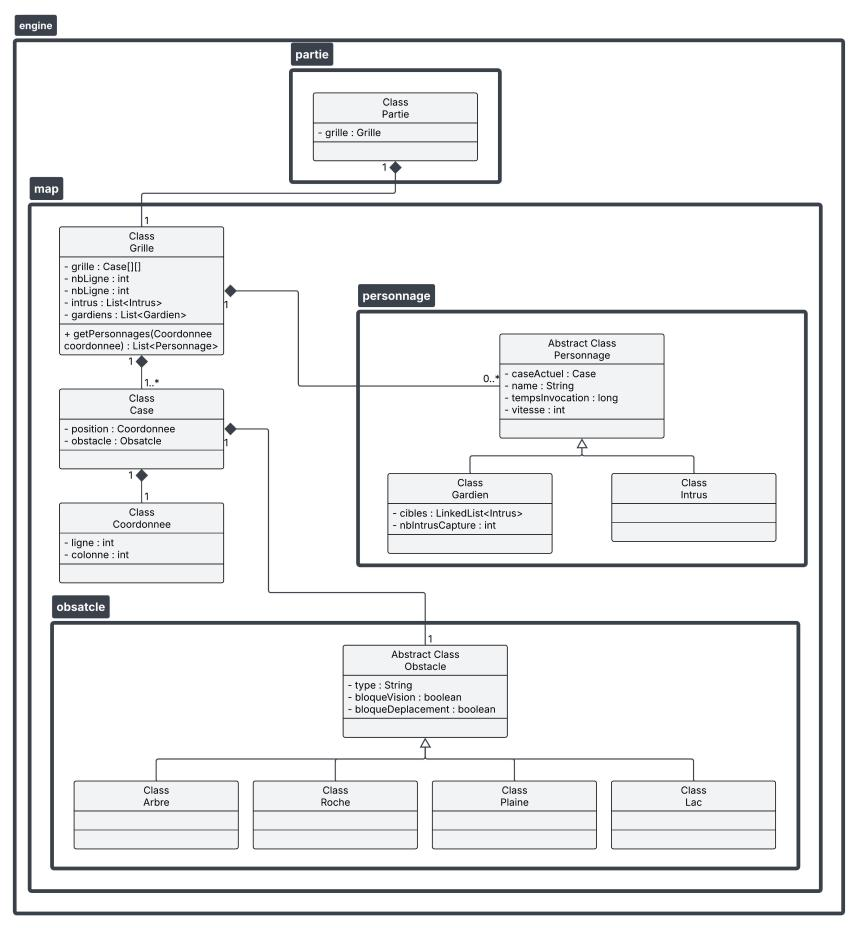
\includegraphics[width=\textwidth]{diag1.jpeg}
        \caption{Diagramme UML global de l’architecture logicielle (MVC)}
        \label{fig:uml-global}
    \end{minipage}
    \hfill
    \begin{minipage}[b]{0.47\textwidth}
        \centering
        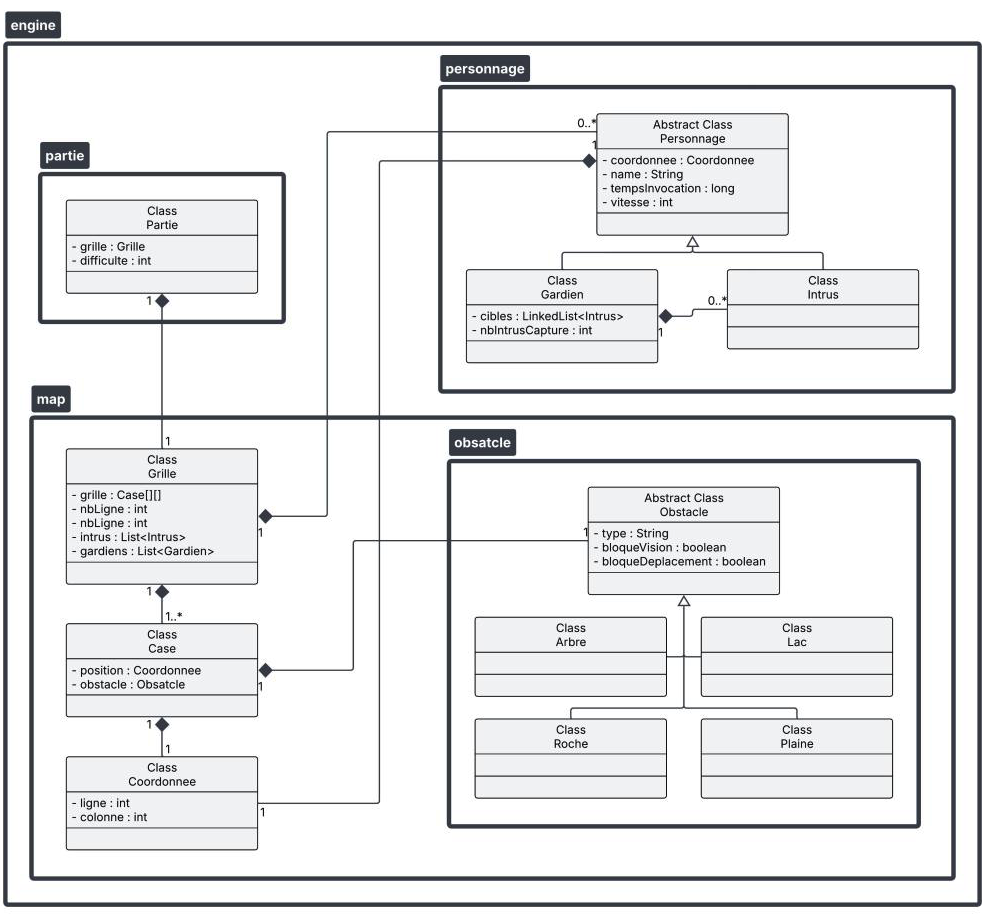
\includegraphics[width=\textwidth]{diag2.png}
        \caption{Diagramme UML du modèle : grille, agents, obstacles}
        \label{fig:uml-modele}
    \end{minipage}
\end{figure}

\vspace{1em}

Ces représentations graphiques ont joué un rôle central dans la conception du projet. Elles nous ont permis :
\begin{itemize}
    \item d’anticiper les interactions entre classes avant d’implémenter le code,
    \item de mieux répartir les responsabilités entre membres de l’équipe,
    \item d’expliquer notre démarche aux encadrants ou au jury de manière synthétique.
\end{itemize}

Elles constituent une base de référence claire pour les sections suivantes, où nous décrivons plus précisément les rôles de chaque couche : le modèle (représentation des entités), le contrôleur (moteur de simulation), et la vue (interface graphique Swing enrichie avec JFreeChart).
\subsection{Couche Modèle : Représentation des entités et de l’environnement}

La couche Modèle est chargée de représenter l’état interne du monde simulé. Elle joue un rôle fondamental en structurant l’ensemble des données sans intégrer de logique décisionnelle ni de traitement graphique. Cette couche assure la modélisation de l’environnement spatial, des entités actives, ainsi que des éléments statiques tels que les obstacles. Elle constitue le socle sur lequel les autres couches (moteur de simulation, interface graphique) vont s’appuyer.

Le moteur est modélisé sous la forme d’une grille 2D, dans laquelle évoluent deux types d'agents dynamiques : les \textbf{gardiens} et les \textbf{intrus}. Chaque agent agit de manière autonome sur cet espace structuré, en interaction avec les obstacles et les autres entités.

La couche Modèle est subdivisée en deux packages :
\begin{itemize}
    \item \texttt{map} : gestion de l’environnement spatial, incluant les coordonnées, les cases, et la structure de la grille ;
    \item \texttt{personne} : représentation des agents actifs, avec leurs propriétés communes et leurs comportements spécifiques.
\end{itemize}
\paragraph{Package \texttt{map} : Grille, Coordonnées, Obstacles }


Ce package regroupe toutes les classes en charge de la définition et de la manipulation de l’espace de simulation.

\paragraph{Classe \texttt{Coordonnee}}

La classe \texttt{Coordonnee} permet de modéliser une position dans la grille en associant deux entiers : une abscisse $x$ (colonne) et une ordonnée $y$ (ligne). Cette encapsulation favorise la clarté du code et limite les erreurs liées aux manipulations directes de couples d’entiers.

\begin{itemize}
    \item \textbf{Attributs} :
    \begin{itemize}
        \item \texttt{int x} : coordonnée en colonne ;
        \item \texttt{int y} : coordonnée en ligne.
    \end{itemize}
    \item \textbf{Méthodes principales} :
    \begin{itemize}
        \item \texttt{equals()} et \texttt{hashCode()} : garantissent une comparaison correcte pour l’utilisation dans des structures de données telles que \texttt{HashSet} et \texttt{HashMap}.
        \item \texttt{voisins()} : calcule et retourne les coordonnées voisines immédiates accessibles (haut, bas, gauche, droite).
        \item \texttt{distance(Coordonnee c)} : calcule la distance de Manhattan entre deux positions, ce qui est essentiel pour évaluer la proximité entre un gardien et un intrus.
    \end{itemize}
    \item \textbf{Responsabilités} :
    \begin{itemize}
        \item Manipulation des positions.
        \item Optimisation des algorithmes de recherche et de mouvement.
    \end{itemize}
\end{itemize}

\vspace{1em}

\paragraph{Classe \texttt{Case}}

La classe \texttt{Case} représente une cellule élémentaire de la grille. Chaque case peut être traversable ou non, visible ou non, et occupée ou non par un agent actif.

\begin{itemize}
    \item \textbf{Attributs} :
    \begin{itemize}
        \item \texttt{boolean obstacle} : indique la présence d’un obstacle (lac, arbre, Roche) ;
        \item \texttt{boolean visible} : indique si la case est actuellement visible par un agent ;
        
        \item \texttt{Personne occupant} : référence vers l’agent occupant la case.
    \end{itemize}
    \item \textbf{Méthodes principales} :
    \begin{itemize}
        \item \texttt{estLibre()} : retourne \texttt{true} si la case est libre (pas d’obstacle ni d’agent).
        \item \texttt{setObstacle(boolean o)} : ajoute ou retire un obstacle sur la case.
        \item \texttt{getAffichage()} : retourne un symbole graphique ou une couleur pour l’affichage, en fonction de l’état de la case.
    \end{itemize}
    \item \textbf{Responsabilités} :
    \begin{itemize}
        \item Support fondamental pour la détection de collision et l’évaluation de la visibilité.
        \item Fournir un support aux calculs de déplacements et aux algorithmes de détection.
    \end{itemize}
\end{itemize}

\vspace{1em}

\paragraph{Classe \texttt{Grille}}

La classe \texttt{Grille} modélise l’espace de simulation global sous la forme d’un tableau 2D de \texttt{Case}.

\begin{itemize}
    \item \textbf{Attributs} :
    \begin{itemize}
        \item \texttt{Case[][] cases} : matrice représentant les cases du monde simulé ;
        \item \texttt{int largeur, int hauteur} : dimensions de la grille.
    \end{itemize}
    \item \textbf{Méthodes principales} :
    \begin{itemize}
        \item \texttt{getCase(Coordonnee c)} : retourne la case correspondant à une coordonnée donnée.
        \item \texttt{estAccessible(Coordonnee c)} : indique si une case est libre d’accès.
        \item \texttt{placerPersonne(Personne p, Coordonnee c)} : place un agent sur une case spécifique.
        \item \texttt{getCasesVisibles(Personne p)} : calcule les cases visibles depuis la position d'un agent, en fonction de son champ de vision et des obstacles présents.
        \item \texttt{reinitialiser()} : remet à zéro l'état des cases (utile lors de la réinitialisation de la simulation).
    \end{itemize}
    \item \textbf{Responsabilités} :
    \begin{itemize}
        \item Centraliser la gestion des interactions spatiales.
        \item Servir d’espace de référence unique pour les déplacements, la visibilité et l’affichage.
    \end{itemize}
\end{itemize}

La \texttt{Grille} est ainsi un composant pivot du modèle : elle structure l’ensemble des interactions physiques possibles entre les agents et l’environnement.

---

\subsubsection{ Package \texttt{personne} : Agents actifs et Comportements de base}

Le package \texttt{personne} regroupe toutes les classes associées aux agents dynamiques présents dans la simulation. Il définit l’architecture commune aux entités actives ainsi que leurs comportements propres.

\paragraph{Classe abstraite \texttt{Personne}}

La classe abstraite \texttt{Personne} définit les attributs fondamentaux partagés par toutes les entités dynamiques, ainsi que les méthodes génériques liées à leur comportement.

\begin{itemize}
    \item \textbf{Attributs} :
    \begin{itemize}
        \item \texttt{Coordonnee position} : position actuelle sur la grille ;
        \item \texttt{int champDeVision} : portée de la visibilité ;
        \item \texttt{Deplacement strategie} : stratégie de déplacement appliquée (aléatoire, poursuite, fuite) ;
        \item \texttt{String couleur} : couleur d'affichage de l'agent.
    \end{itemize}
    \item \textbf{Méthodes principales} :
    \begin{itemize}
        \item \texttt{seDeplacer(Grille grille)} : effectue un déplacement en appliquant la stratégie associée.
        \item \texttt{getZoneVisible(Grille grille)} : retourne la liste des cases visibles selon le champ de vision de l’agent et les obstacles présents.
        \item \texttt{estIntrus()} : méthode permettant de distinguer s’il s’agit d’un intrus ou d’un gardien.
    \end{itemize}
    \item \textbf{Responsabilités} :
    \begin{itemize}
        \item Normaliser la gestion des déplacements et de la visibilité.
        \item Garantir un comportement cohérent pour l'ensemble des agents dynamiques.
    \end{itemize}
\end{itemize}

\vspace{1em}

\paragraph{Classe \texttt{Gardien}}

La classe \texttt{Gardien} hérite de \texttt{Personne}. Elle représente les entités de surveillance actives dans la grille.

\begin{itemize}
    \item \textbf{Comportements} :
    \begin{itemize}
        \item Patrouille aléatoire lorsque aucun intrus n’est détecté.
        \item Activation de la poursuite dès qu'un intrus est repéré dans son champ de vision.
    \end{itemize}
    \item \textbf{Spécificité} :
    \begin{itemize}
        \item Interaction forte avec l’environnement : analyse en permanence des zones visibles pour ajuster le comportement.
    \end{itemize}
\end{itemize}

\vspace{1em}

\paragraph{Classe \texttt{Intrus}}

La classe \texttt{Intrus} modélise les agents furtifs cherchant à éviter toute détection.

\begin{itemize}
    \item \textbf{Comportements} :
    \begin{itemize}
        \item Se déplacer en priorité vers les zones non visibles ;
        \item Modifier de manière réactive leur direction lorsqu’un danger est détecté.
    \end{itemize}
    \item \textbf{Spécificité} :
    \begin{itemize}
        \item Capacité d’adaptation immédiate à la détection l'intrus, favorisant la survie dans l’environnement hostile.
    \end{itemize}
\end{itemize}

\vspace{1em}
\subsubsection{ Gestion centrale des entités : \texttt{PersonnageManager}}

La classe \texttt{PersonnageManager} joue un rôle fondamental dans la simulation. Elle est responsable de la \textbf{gestion globale des personnages} (gardiens et intrus) présents sur la grille. Son architecture suit le principe du \textbf{singleton}, garantissant qu’une seule instance coordonne l’ensemble des agents.

\vspace{1em}
\paragraph{Responsabilités principales}
\begin{itemize}
    \item Initialiser, ajouter et retirer dynamiquement les agents (\texttt{Gardiens} et \texttt{Intrus}).
    \item Contrôler les déplacements, observer l'environnement, et mettre à jour l’état des agents à chaque tour de simulation.
    \item Assurer la communication d’informations stratégiques (ex : transmission de la position d’un intrus détecté entre gardiens).
    \item Gérer le \textbf{gardien actif} si le joueur contrôle un personnage manuellement.
    \item Maintenir le nombre d’intrus constant 
\end{itemize}

\vspace{1em}
\paragraph{Structure de la classe}
\begin{itemize}
    \item \textbf{Attributs principaux} :
    \begin{itemize}
        \item \texttt{List<Personnage> personnages} : Liste dynamique contenant tous les agents (gardiens et intrus).
        \item \texttt{Grille grille} : Référence vers l’environnement spatial.
        \item \texttt{Gardien gardienActif} : Gardien contrôlé manuellement (optionnel).
        \item \texttt{int nbIntrusInitial, nbGardienInitial} : Suivi des effectifs initiaux pour la simulation.
        \item \texttt{int nbIntrusCapture} : Compteur d’intrus capturés pendant la simulation.
    \end{itemize}
    \item \textbf{Singleton} :
    \begin{itemize}
        \item Instancié via \texttt{initInstance(Grille, Settings)}, récupérable avec \texttt{getInstance()}.
    \end{itemize}
\end{itemize}

\vspace{1em}
\paragraph{Cycle de vie des personnages}

À chaque cycle  de la simulation, la méthode \texttt{actionPersonnages()} est appelée. Elle organise les étapes suivantes :
\begin{enumerate}
    \item \textbf{Déplacement des intrus} : les intrus se déplacent selon leur stratégie (aléatoire ou stratégique).
    \item \textbf{Observation des intrus} : chaque intrus analyse son environnement.
    \item \textbf{Déplacement des gardiens} : les gardiens avancent en suivant leur propre stratégie (aléatoire ou poursuite).
    \item \textbf{Observation des gardiens} : les gardiens observent leur environnement pour repérer des intrus.
    \item \textbf{Communication} : si un gardien détecte un intrus, il transmet cette information aux autres gardiens proches.
    \item \textbf{Respawn des intrus} : s’il manque des intrus par rapport au nombre initial, de nouveaux intrus sont créés.
\end{enumerate}

\vspace{1em}
\paragraph{Gestion des déplacements}

Chaque agent (gardien ou intrus) possède une stratégie de déplacement associée via une \textbf{factory} (\texttt{DeplacementFactory}).  
Cette stratégie peut être :
\begin{itemize}
    \item \textbf{Déplacement aléatoire} : choisir un voisin libre au hasard.
    \item \textbf{Déplacement stratégique} : se rapprocher d'une cible détectée.
    \item \textbf{Déplacement manuel} : contrôlé par l'utilisateur.
\end{itemize}

Lorsqu'un personnage est créé (par \texttt{ajouterGardien()} ou \texttt{ajouterIntrus()}), sa stratégie par défaut est définie automatiquement.

\vspace{1em}
\paragraph{Observation et communication entre agents}

Lorsqu'un gardien observe, il récupère une liste d'entités visibles grâce à son algorithme de champ de vision :
\begin{itemize}
    \item S'il repère des intrus, il adapte sa stratégie pour les poursuivre.
    \item S'il a l'option de communication activée, il partage cette information aux gardiens voisins, leur permettant de viser également l'intrus détecté.
\end{itemize}

\vspace{1em}
\paragraph{Respawn et maintien de la simulation}

Si l’option est activée dans les paramètres, la méthode \texttt{reSpawnIntrus()} vérifie après chaque tick s’il manque des intrus par rapport au nombre initial. En cas de déficit :
\begin{itemize}
    \item Un nouvel intrus est généré aléatoirement sur une case libre.
    \item Ceci assure une simulation continue et maintient un défi constant pour les gardiens.
\end{itemize}

\vspace{1em}
\paragraph{Gestion du Gardien Actif}

Un agent spécifique peut être contrôlé manuellement (le \texttt{gardienActif}). 
\begin{itemize}
    \item Lors de l’activation, sa stratégie de déplacement est remplacée par \texttt{DéplacementManuel}.
    \item Lors de la désactivation, il repasse en déplacement automatique par défaut.
\end{itemize}
Cela permet des tests interactifs ou des modes de jeu semi-automatisés.

\vspace{1em}
\paragraph{journalisation}

Le \texttt{PersonnageManager} utilise un système de journalisation (\texttt{LoggerUtility}) pour :
\begin{itemize}
    \item Suivre l’ajout et la suppression de personnages.
    \item Détecter les erreurs (par exemple, tentative de suppression d’un agent inexistant).
    \item Documenter les événements majeurs (capture d'intrus, observations, communications entre agents).
\end{itemize}
Cette approche rend la simulation plus traçable, robuste et fiable.

\bigskip
\paragraph{Résumé}
Le \texttt{PersonnageManager} est le véritable \textbf{chef d’orchestre} de la simulation :
\begin{itemize}
    \item Il coordonne tous les agents, leurs déplacements et leurs interactions.
    \item Il contrôle les événements dynamiques du jeu de manière centralisée.
    \item Il s’adapte aux configurations de la simulation (nombre d’intrus, respawn, communication).
\end{itemize}
C’est un composant essentiel, garantissant la fluidité et la cohérence du monde simulé à chaque itération du moteur.


\subsubsection{ Interface \texttt{Deplacement}}

L'interface \texttt{Deplacement} définit un contrat standard pour toutes les stratégies de mouvement.  
Chaque agent peut ainsi déléguer son calcul de déplacement à une instance spécifique de \texttt{Deplacement}.

\paragraph{Méthodes définies :}
\begin{itemize}
    \item \texttt{Coordonnee calculerProchainePosition(Personne p, Grille g)} : détermine la prochaine position cible pour l'agent donné dans la grille.
    \item \texttt{void changerStrategie()} (optionnelle) : permet, par exemple, de modifier dynamiquement la stratégie lorsqu'une situation évolue (par exemple lors de la détection d'un intrus).
\end{itemize}

\paragraph{Objectifs :}
\begin{itemize}
    \item Découpler la logique de déplacement du reste du moteur.
    \item Permettre le changement dynamique de comportement pour un agent.
    \item Favoriser l'extensibilité du système en permettant l’ajout de nouvelles stratégies.
\end{itemize}
\subsubsection{ Classe \texttt{DeplacementAleatoire}}

Cette stratégie correspond à un déplacement \textbf{naïf et non informé}.

\paragraph{Principe :}
\begin{itemize}
    \item L’agent choisit aléatoirement l’une des cases accessibles autour de lui (haut, bas, gauche, droite).
    \item Aucune prise en compte de l’environnement global, seulement la liberté locale immédiate.
    \item Le déplacement est immédiat si la case ciblée est valide ; sinon, aucune action n'est entreprise pour ce tour.
\end{itemize}

\paragraph{Implémentation :}
\begin{itemize}
    \item La classe \texttt{DeplacementAleatoire} hérite de \texttt{StrategieDeplacement}.
    \item Elle utilise un tableau contenant toutes les directions possibles (\texttt{Direction.values()}).
    \item À chaque itération :
    \begin{enumerate}
        \item Un entier aléatoire est tiré pour choisir une direction.
        \item La direction du personnage est mise à jour pour changer son animation visuelle.
        \item La nouvelle coordonnée est calculée en fonction de cette direction.
        \item La validité de la case cible est vérifiée grâce à la méthode \texttt{isCoordonneeValide()}.
        \item Si valide, la position du personnage est mise à jour sur la grille.
        \item Un éventuel contact avec un autre agent est ensuite vérifié (\texttt{contactPersonnage()}).
    \end{enumerate}
\end{itemize}

\paragraph{Utilisation :}
\begin{itemize}
    \item Comportement par défaut des \texttt{Intrus} non détectés.
    \item Comportement des \texttt{Gardiens} en phase de patrouille libre sans alerte active.
\end{itemize}


\paragraph{Algorithme détaillé :}
\begin{verbatim}
1. Récupérer la position actuelle de l'agent (x, y).
2. Générer la liste des coordonnées voisines accessibles (haut, bas, gauche, droite).
3. Filtrer les cases libres (sans obstacle ni occupant).
4. Choisir aléatoirement une case parmi les candidates.
5. Retourner la position choisie.
\end{verbatim}



\subsubsection{ Classe \texttt{DeplacementStrategique}}

Cette stratégie vise à déplacer l'agent de manière \textbf{stratégique} vers un \textbf{objectif détecté} (par exemple, un intrus visible).

\paragraph{Principe :}
\begin{itemize}
    \item L’agent choisit systématiquement la case voisine qui le rapproche le plus de sa cible (stratégie ).
    
\end{itemize}

\paragraph{Utilisation :}
\begin{itemize}
    \item Activation immédiate par les \texttt{Gardiens} dès qu’un intrus entre dans leur champ de vision.
\end{itemize}

\paragraph{Algorithme détaillé :}
\begin{verbatim}
1. Identifier les intrus visibles depuis la position de l'agent.
2. Sélectionner l'intrus le plus proche en distance ou dans son champ de visiosions.
3. Pour chaque case voisine accessible :
   a. Calculer la distance à l'intrus cible.
   b. Mémoriser la case minimisant cette distance.
4. Se déplacer vers la case retenue.
\end{verbatim}

\paragraph{Limites :}
\begin{itemize}
    \item Peut être bloqué par des obstacles si la cible n'est pas directement accessible.
    \item Ne prévoit pas de chemin global optimal (pas d'anticipation des détours).
\end{itemize}

\paragraph{Améliorations futures possibles :}
\begin{itemize}
    \item Intégration d’un algorithme de pathfinding global ( Dijkstra) pour contourner les obstacles complexes.
    \item Ajout d’une prise en compte des dangers pour éviter les zones à risque.
\end{itemize}
\subsubsection{ Classe \texttt{DeplacementManuel}}

Cette stratégie permet un \textbf{contrôle manuel} d'un agent par l'utilisateur via l'IHM graphique.

\paragraph{Principe général :}
\begin{itemize}
    \item L'agent lit sa direction courante définie par l'utilisateur.
    \item Il calcule sa prochaine position en fonction de cette direction.
    \item Il vérifie que la case visée est accessible.
    \item Il se déplace uniquement si la case est valide.
    \item Après déplacement, il vérifie les éventuels contacts avec d'autres agents (ex: capture d'intrus).
\end{itemize}

\paragraph{Cycle complet de déplacement :}
\begin{enumerate}
    \item Lire la direction assignée à l'agent (\texttt{Direction}).
    \item Vérifier que la direction n'est pas nulle.
    \item Mettre à jour l'animation graphique pour correspondre au mouvement.
    \item Calculer la nouvelle coordonnée en fonction de la direction.
    \item Tester la validité de la nouvelle case via la grille (\texttt{Grille.isCoordonneeValide()}).
    \item Si la case est libre, déplacer l'agent.
    \item Réinitialiser l'animation.
    \item Vérifier la présence de contacts (collision entre gardien et intrus).
\end{enumerate}

\paragraph{Cas d'utilisation :}
\begin{itemize}
    \item Mode "manuel" pour piloter un Gardien et capturer les Intrus.
    \item Contrôle direct par l'utilisateur via le clavier (touches directionnelles).
\end{itemize}


\paragraph{Remarque :}
Cette stratégie ne calcule aucun chemin optimal ni n'évite activement les obstacles :
le déplacement est \textbf{entièrement} sous la responsabilité de l'utilisateur.

\subsubsection{ Classe \texttt{DeplacementPoursuite}}

Cette stratégie permet aux \texttt{Gardiens} de \textbf{poursuivre activement} les \texttt{Intrus} détectés dans leur environnement.

\paragraph{Principe général :}
\begin{itemize}
    \item Le gardien tente de localiser un intrus accessible dans sa liste de cibles.
    \item Si une cible est trouvée et accessible, un chemin est calculé jusqu'à sa position.
    \item Le gardien suit le chemin pas à pas pour se rapprocher de la cible.
    \item En absence de cible valide, un déplacement aléatoire est effectué.
\end{itemize}

\paragraph{Méthodologie de calcul du chemin :}
\begin{enumerate}
    \item Initialiser une exploration à partir de la position actuelle du gardien.
    \item À chaque itération (pas), explorer les cases adjacentes accessibles.
    \item Si l'intrus est trouvé dans les cases adjacentes, considérer le chemin comme accessible.
    \item Reconstruire le chemin optimal en remontant les couches d'exploration.
    \item Inverser le chemin pour obtenir un parcours du gardien vers l'intrus.
\end{enumerate}

\paragraph{Gestion des cas d'échec :}
\begin{itemize}
    \item Si aucun chemin viable n'est trouvé (\texttt{CheminNonViable}), la cible est retirée.
    \item Le gardien tente alors de poursuivre la cible suivante dans sa liste.
    \item Si aucune cible n'est atteignable, il effectue un déplacement aléatoire.
\end{itemize}

\paragraph{Fonctions principales :}
\begin{itemize}
    \item \texttt{deplacer(Personnage)} : Méthode principale de déplacement intelligent.
    \item \texttt{cibleAccessible(Gardien)} : Vérifie la validité d'une cible.
    \item \texttt{trouverChemin(Intrus)} : Reconstruit le chemin du gardien vers l'intrus.
    \item \texttt{deplacerVersCible(Gardien, Intrus)} : Effectue le mouvement vers l'intrus.
\end{itemize}

\paragraph{Cas d'utilisation :}
\begin{itemize}
    \item Simulation de patrouilles actives.
    \item Systèmes de surveillance où les agents doivent intercepter rapidement les intrus.
\end{itemize}

\paragraph{Remarque :}
L'utilisation de logs détaillés (\texttt{LoggerUtility}) permet une traçabilité complète du comportement du gardien dans la poursuite.

\paragraph{Stratégie Générique de Déplacement : \texttt{StrategieDeplacement}}

La classe abstraite \texttt{StrategieDeplacement} constitue la base commune de toutes les stratégies de mouvement des agents (gardiens et intrus).  
Elle définit des outils standards pour :
\begin{itemize}
    \item Gérer les informations essentielles au déplacement ;
    \item Coordonner les interactions avec l’environnement (\texttt{Grille}) ;
    \item Mettre à jour l'animation des personnages ;
    \item Détecter les collisions entre agents (gardien/intrus).
\end{itemize}

\vspace{1em}
\paragraph{Responsabilités principales}
\begin{itemize}
    \item Fournir un accès direct à la grille (\texttt{Grille}) et aux personnages (\texttt{PersonnageManager}).
    \item Gérer la logique de \textbf{contact} : lorsqu’un \texttt{Gardien} et un \texttt{Intrus} occupent la même case, l’intrus est capturé.
    \item Actualiser les \textbf{animations visuelles} des personnages lorsqu'ils changent de direction.
\end{itemize}

\vspace{1em}
\paragraph{Structure et Attributs}
\begin{itemize}
    \item \texttt{Grille grille} : référence à la carte du monde pour connaître les obstacles et les déplacements valides.
    \item \texttt{PersonnageManager personnages} : accès centralisé à tous les agents présents sur la grille.
\end{itemize}

Ces deux références sont essentielles pour permettre aux stratégies concrètes (aléatoire, stratégique, manuel) d’interagir avec le monde et ses entités.

\vspace{1em}
\paragraph{Méthodes principales}
\begin{itemize}
    \item \textbf{\texttt{updateAnimation(Personnage, Direction)}} : 
    \begin{itemize}
        \item Met à jour l'orientation (\texttt{Direction}) du personnage.
        \item Déclenche une animation visuelle pour rendre les déplacements fluides et réalistes.
    \end{itemize}
    \item \textbf{\texttt{contactPersonnage(Coordonnee)}} :
    \begin{itemize}
        \item Détecte s’il y a à la même position au moins un \texttt{Gardien} et un \texttt{Intrus}.
        \item Si c'est le cas :
        \begin{enumerate}
            \item L'intrus est retiré de la grille (capture).
            \item Le gardien qui a capturé augmente son compteur d’intrus capturés.
        \end{enumerate}
        \item Ce mécanisme est automatique : il est déclenché dès qu'un déplacement est effectué.
    \end{itemize}
\end{itemize}

\vspace{1em}
\paragraph{Constructeur}

Le constructeur de la classe reçoit deux paramètres :
\begin{itemize}
    \item La \texttt{Grille} sur laquelle le déplacement a lieu.
    \item Le \texttt{PersonnageManager} contenant la liste de tous les agents.
\end{itemize}
Ces deux dépendances sont nécessaires pour permettre à toutes les sous-classes (déplacement aléatoire, stratégique, manuel) d’effectuer leurs calculs de manière cohérente.

\vspace{1em}
\paragraph{Rôle Architectural}

La classe \texttt{StrategieDeplacement} joue un double rôle :
\begin{itemize}
    \item Elle sert de \textbf{socle commun} pour éviter la duplication de code entre différentes stratégies.
    \item Elle garantit que toutes les stratégies peuvent :
    \begin{enumerate}
        \item Accéder facilement aux informations du monde ;
        \item Détecter des événements comme la capture d’intrus ;
        \item Mettre à jour visuellement les agents.
    \end{enumerate}
\end{itemize}

Grâce à cette abstraction, l’ajout de nouvelles stratégies devient simple : il suffit d’étendre \texttt{StrategieDeplacement} et d’implémenter la méthode de calcul du déplacement.

\bigskip
\paragraph{Résumé}
\texttt{StrategieDeplacement} est la pierre angulaire qui :
\begin{itemize}
    \item Facilite l’écriture de comportements de mouvement diversifiés ;
    \item Centralise les tâches communes (contact, animation) pour toutes les stratégies ;
    \item Contribue fortement à l’extensibilité et à la propreté architecturale du moteur de simulation.
\end{itemize}

\subsubsection{ Classe \texttt{DeplacementFactory}}

La classe \texttt{DeplacementFactory} constitue une fabrique centralisée (pattern \textit{Factory}) chargée de produire les différentes stratégies de déplacement utilisées par les agents (Gardiens et Intrus).

Elle est indispensable pour garantir :
\begin{itemize}
    \item Une création uniforme et contrôlée des objets de type \texttt{Deplacement}.
    \item Une réutilisation des instances lorsque cela est possible, afin d’éviter des créations inutiles (optimisation mémoire et performances).
\end{itemize}

\paragraph{Responsabilités principales}
\begin{itemize}
    \item Fournir une méthode unique \texttt{getDeplacement(String type, PersonnageManager, Grille)} permettant d’obtenir une stratégie de mouvement.
    \item Cacher la logique complexe d’instanciation aux autres classes du moteur.
    \item Gérer un \textbf{cache} d’instances pour certains types de déplacements standard (par exemple, aléatoire, manuel).
\end{itemize}

\vspace{1em}
\paragraph{Fonctionnement interne}

\begin{itemize}
    \item Un attribut \texttt{private static Map<String, Deplacement> deplacements} conserve les stratégies déjà créées.
    \item Lorsqu'une stratégie est demandée via \texttt{getDeplacement} :
    \begin{enumerate}
        \item Si elle existe déjà dans la carte, elle est retournée directement (\textbf{singleton interne} pour chaque type).
        \item Sinon, une nouvelle instance est créée, enregistrée dans la carte, puis retournée.
    \end{enumerate}
\end{itemize}

\vspace{1em}
\paragraph{Types de déplacements gérés}

\begin{itemize}
    \item \texttt{Aleatoire} : déplacement aléatoire simple (exploration sans but).
    \item \texttt{Manuel} : contrôle direct par un utilisateur (via clavier ou souris).
    \item \texttt{Poursuite} : déplacement dirigé de manière offensive vers une cible visible (gardien poursuivant un intrus).
    \item \texttt{Case} : déplacement case par case basé sur des calculs de proximité (approche basique sans poursuite avancée).
\end{itemize}

Chaque type correspond à une classe spécifique :
\begin{itemize}
    \item \texttt{DeplacementAleatoire}
    \item \texttt{DeplacementManuel}
    \item \texttt{DeplacementPoursuite}
    \item \texttt{DeplacementCase}
\end{itemize}

\vspace{1em}
\paragraph{Exemple typique d'utilisation}

Lorsqu'un agent détecte un événement spécial (ex: un intrus est repéré par un gardien), il peut automatiquement changer de comportement :


Grâce à la \texttt{DeplacementFactory}, le moteur de simulation reste souple et peut adapter dynamiquement les comportements sans devoir gérer manuellement la création d'objets.

\vspace{1em}
\paragraph{Gestion des erreurs }

\begin{itemize}
    \item Si un type inconnu est demandé, la factory retourne par défaut une stratégie \texttt{Aleatoire}.
    \item Cette approche prévient les plantages tout en assurant une continuité de la simulation.
    \item Des messages de log (\texttt{Logger}) sont générés à chaque demande de stratégie pour faciliter le débogage.
\end{itemize}

\vspace{1em}
\paragraph{Résumé}

La \texttt{DeplacementFactory} joue un rôle clé dans la gestion intelligente des comportements d'agents :
\begin{itemize}
    \item Centralisation de la création d’objets de stratégie ;
    \item Optimisation des ressources (réutilisation des instances) ;
    \item Robustesse face aux erreurs de type ;
    \item Simplicité d’extension : il suffit d’ajouter un nouveau type dans la méthode \texttt{getDeplacement}.
\end{itemize}
Elle est donc indispensable à la flexibilité et à l’évolutivité du moteur de simulation.

\subsubsection{ Moteur de Simulation }

La simulation fonctionne selon un moteur discret : chaque cycle (tick) correspond à une unité de temps durant laquelle tous les agents agissent une seule fois.

\paragraph{Déroulement d’un cycle de simulation :}
\begin{enumerate}
    \item Réinitialisation des états visuels de la grille.
    \item Pour chaque agent :
    \begin{itemize}
        \item Calcul du champ de vision actuel.
        \item Évaluation des menaces/opportunités ;
        \item Changement de stratégie si nécessaire ;
        \item Calcul de la prochaine position via \texttt{calculerProchainePosition()} ;
        \item Validation et exécution du déplacement.
    \end{itemize}
    \item Vérification des captures : un intrus et un gardien occupant la même case entraîne l'élimination de l'intrus.
    \item Rafraîchissement de l’interface graphique.
\end{enumerate}

\paragraph{Avantages :}
\begin{itemize}
    \item Simulation déterministe, facile à analyser et à déboguer.
    \item Gestion simplifiée des actions concurrentes entre agents.
    \item Possibilité de rejouer les parties pour analyser le comportement des stratégies.
\end{itemize}

\subsubsection{ Algorithme de Champ de Vision }

La perception visuelle des agents est fondamentale pour influencer leurs décisions.
\paragraph{Méthode de calcul utilisée :}

La détection visuelle d'un agent (gardien ou intrus) repose sur un balayage systématique d'un carré centré autour de sa position, dont la taille dépend directement de son rayon de vision $r$. L'algorithme est structuré de la manière suivante :

\begin{itemize}
    \item \textbf{Définition du champ de vision} : 
    \begin{itemize}
        \item Construire un carré de taille $(2r+1) \times (2r+1)$ centré sur la position actuelle de l'agent.
        \item Chaque case de ce carré correspond à une position potentiellement visible par l'agent.
    \end{itemize}
    \item \textbf{Analyse de visibilité} : 
    \begin{itemize}
        \item Pour chaque case du carré :
        \begin{itemize}
            \item Tracer virtuellement une ligne droite entre la position de l'agent et la case considérée.
            \item Parcourir cette ligne et détecter la présence éventuelle d'obstacles (obstacles de type mur, lac, arbre, roche).
        \end{itemize}
    \end{itemize}
    \item \textbf{Gestion des obstacles} :
    \begin{itemize}
        \item Dès qu'un obstacle bloquant est détecté le long de cette ligne :
        \begin{itemize}
            \item La visibilité de cette case est arrêtée.
            \item Aucune case située au-delà de l'obstacle dans cette direction n'est considérée comme visible.
        \end{itemize}
    \end{itemize}
\end{itemize}



\paragraph{Justification du choix de l'algorithme :}

Cette approche basée sur un balayage discret ligne par ligne permet :
\begin{itemize}
    \item d'obtenir une vision réaliste limitée par les obstacles du terrain,
    
    \item d'assurer que la vision soit bloquée de manière réaliste par des éléments du décor (par exemple, impossible de voir à travers un lac ou un arbre épais).
\end{itemize}

    

\paragraph{Considérations :}
\begin{itemize}
    \item Les obstacles denses réduisent fortement les champs de vision.
    \item Le champ de vision est recalculé à chaque tick, ce qui nécessite une implémentation efficace pour conserver de bonnes performances.
\end{itemize}

---
\section{Couche Interface Graphique : Visualisation et Interaction Utilisateur}

La couche graphique constitue la \textbf{porte d'entrée visuelle} de la simulation.  
Elle permet de \textbf{représenter en temps réel} l'évolution du système, de \textbf{visualiser} les agents (gardiens, intrus), \textbf{d'interagir} avec eux, et d'\textbf{influencer la simulation} via le clavier et la souris.

Cette interface repose exclusivement sur \texttt{Swing}, la bibliothèque graphique de Java, connue pour sa \textbf{flexibilité}, sa \textbf{portabilité}, et sa \textbf{capacité de customisation}.

L'objectif de cette couche est double :
\begin{itemize}
    \item Offrir une \textbf{visualisation claire} et \textbf{fluide} du déroulement de la simulation.
    \item Permettre une \textbf{interaction intuitive} de l'utilisateur avec les agents et l'environnement.
\end{itemize}

Elle suit une architecture \textbf{modulaire} et \textbf{couche par couche}, permettant des évolutions futures (ajout de nouveaux types d’affichage, intégration de nouveaux comportements graphiques).

\bigskip

\subsection{ Classe \texttt{MainGUI}}

\paragraph{Rôle :}  
La classe \texttt{MainGUI} est la \textbf{classe principale} de l’interface utilisateur.  
Elle :
\begin{itemize}
    \item Initialise la fenêtre principale (\texttt{JFrame}).
    \item Installe les composants graphiques : grille de jeu, menu, panneau latéral.
    \item Lance et pilote la boucle de simulation.
\end{itemize}

\paragraph{Structure interne :}
\begin{itemize}
    \item \textbf{GameDisplay} : Panneau central où la simulation est dessinée.
    \item \textbf{SidePanel} : Panneau latéral avec les informations dynamiques.
    \item \textbf{MenuBar} : Menu de contrôle (démarrer, pause, options...).
    \item \textbf{ChronoSimulation} : Gestion du temps et de la vitesse de simulation.
\end{itemize}

\paragraph{Méthodes clés :}
\begin{itemize}
    \item \texttt{init()} : Crée tous les éléments graphiques et configure l'affichage.
    \item \texttt{run()} : Boucle de jeu principale : rafraîchit la simulation à intervalle régulier.
    \item \texttt{setActive()} : Active ou met en pause l'évolution de la simulation.
\end{itemize}

\paragraph{Connexion au moteur :}
\begin{itemize}
    \item MainGUI utilise \textbf{PersonnageManager} pour interagir avec les agents.
    \item Elle contrôle la simulation en appelant des méthodes sur le moteur (action, génération de grille, etc.).
    \item Elle est \textbf{observatrice passive} du modèle : elle ne fait que redessiner les états modifiés.
\end{itemize}

\paragraph{Justification :}
La séparation stricte entre \textbf{affichage} (MainGUI) et \textbf{modèle} (Grille, PersonnageManager) garantit une \textbf{architecture MVC claire}, favorisant la maintenance et l'extensibilité du code.

\bigskip

\subsection{Classe \texttt{GameDisplay}}

\paragraph{Rôle :}  
\texttt{GameDisplay} est le \textbf{conteneur graphique} principal.  
Il héberge la stratégie d’affichage \texttt{PaintStrategy}, qui orchestre le dessin de tous les éléments visibles.

\paragraph{Fonctionnement interne :}
\begin{itemize}
    \item Hérite de \texttt{JPanel}.
    \item Redéfinit \texttt{paintComponent(Graphics g)} pour déclencher le rendu de la simulation.
    \item Dépend de \textbf{PaintStrategy} pour décider \textbf{quoi dessiner} et \textbf{dans quel ordre}.
\end{itemize}

\paragraph{Connexion avec les événements utilisateur :}
\begin{itemize}
    \item Ajoute des \texttt{MouseListener} et \texttt{KeyListener} pour détecter les actions de l’utilisateur sur la grille.
    \item Détecte les clics sur les cases pour sélectionner un agent.
    \item Permet de piloter un agent activement par les touches du clavier.
\end{itemize}

\paragraph{Justification :}
Cette classe isole les responsabilités :
\begin{itemize}
    \item \textbf{GameDisplay} : Conteneur simple (gère la dimension et la répartition).
    \item \textbf{PaintStrategy} : Se charge du dessin lui-même.
\end{itemize}
Cela permet une meilleure \textbf{lisibilité}, une \textbf{meilleure évolutivité}, et une gestion plus facile des effets d’affichage (zoom, overlays, etc.).

\bigskip

\subsection{Classe \texttt{PaintStrategy}}

\paragraph{Rôle :}  
\texttt{PaintStrategy} est la \textbf{stratégie de rendu} de l’interface graphique.  
Elle décide \textbf{quels éléments dessiner} et \textbf{dans quel ordre}, en respectant les priorités visuelles.

\paragraph{Structure interne :}
\begin{itemize}
    \item Contient une liste de classes \texttt{Dessiner} (interface) représentant différents éléments :
    \begin{itemize}
        \item \texttt{DessinerGrille} : affichage de la carte et des obstacles.
        \item \texttt{DessinerPersonnages} : affichage des gardiens et des intrus.
        \item \texttt{DessinerVision} : affichage des zones de vision (optionnel).
        \item \texttt{DessinerDeplacement} : affichage des chemins de déplacement (optionnel).
    \end{itemize}
    \item Chaque dessin peut être \textbf{activé/désactivé} indépendamment.
    \item Certains dessins peuvent passer en \textbf{mode performance} (affichage simplifié pour accélérer le rendu).
\end{itemize}

\paragraph{Cycle de dessin :}
\begin{enumerate}
    \item Dessiner la grille (sols, obstacles).
    \item Dessiner les agents (gardiens, intrus).
    \item Dessiner les champs de vision (si activés).
    \item Dessiner les chemins de déplacement (si activés).
\end{enumerate}

\paragraph{Gestion dynamique :}
\begin{itemize}
    \item \texttt{setDessinActif(String nom, boolean etat)} : active/désactive un dessin optionnel.
    \item \texttt{setPerformanceActif(String nom, boolean etat)} : active/désactive le mode simplifié.
\end{itemize}

\paragraph{Justification :}
En séparant les couches d’affichage, on peut :
\begin{itemize}
    \item Ajouter de nouveaux effets visuels facilement.
    \item Modifier dynamiquement ce qui est visible (vision, déplacements…).
    \item Optimiser les performances pour les grandes cartes.
\end{itemize}

\bigskip

\subsection{Interaction avec Swing : Événements Utilisateur}

\paragraph{Types d’événements gérés :}
\begin{itemize}
    \item \textbf{ActionListener} : boutons de contrôle (Démarrer, Pause, Réinitialiser, Options...).
    \item \textbf{MouseListener} : clic sur un agent, clic pour définir un objectif.
    \item \textbf{KeyListener} : contrôle manuel d'un gardien (flèches directionnelles ou ZQSD).
\end{itemize}

\paragraph{Cycle d'interaction typique :}
\begin{enumerate}
    \item L'utilisateur déclenche une action (clic, touche).
    \item Un événement est capturé (ActionEvent, MouseEvent, KeyEvent).
    \item Le moteur de simulation modifie l'état du modèle.
    \item \texttt{repaint()} est appelé pour rafraîchir l’affichage via \texttt{PaintStrategy}.
\end{enumerate}

\paragraph{Justification :}
Grâce à cette architecture basée sur les \textbf{listeners Swing}, l’interface est :
\begin{itemize}
    \item \textbf{Réactive} : répond immédiatement aux actions utilisateur.
    \item \textbf{Extensible} : facile à enrichir avec de nouveaux types d’actions.
    \item \textbf{Synchronisée} : garantit une mise à jour cohérente entre le modèle et la vue.
\end{itemize}

\bigskip

\section*{Conclusion}

La couche interface graphique est \textbf{fondamentale} pour l’expérience utilisateur.  
Elle assure à la fois :
\begin{itemize}
    \item Une \textbf{visualisation intuitive et fluide} de la simulation.
    \item Une \textbf{interaction facile et rapide} avec les agents.
\end{itemize}

Grâce à une conception \textbf{modulaire}, \textbf{séparée} et \textbf{optimisée}, elle offre une grande \textbf{extensibilité} pour :
\begin{itemize}
    \item Ajouter un zoom dynamique ;
    \item Intégrer des affichages stratégiques (réseaux de vision, cartes thermiques) ;
    \item Créer des modes de visualisation avancés (mode multijoueur, replay, etc.).
\end{itemize}

Cette architecture renforce la \textbf{qualité logicielle} générale du projet, en rendant l'application \textbf{facile à maintenir}, \textbf{évolutive} et \textbf{pérenne}.

\subsection*{Conclusion de l’architecture logicielle}

L’architecture logicielle mise en œuvre dans ce projet repose sur une séparation claire des responsabilités entre les couches de données (\textbf{Modèle}), de logique métier (\textbf{Moteur}), et d’affichage (\textbf{Interface graphique}). Ce découpage inspiré du modèle MVC nous a permis de concevoir un système modulaire, extensible, et maintenable.

Chaque classe a été pensée selon les principes de la programmation orientée objet : encapsulation des données, séparation des préoccupations, usage judicieux de l’héritage et du polymorphisme. La couche \textbf{Modèle} structure l’environnement et les agents de manière robuste ; la couche \textbf{Moteur} permet une simulation déterministe, avec une flexibilité stratégique offerte par le design pattern \texttt{Strategy} ; enfin, la couche \textbf{Vue} offre un affichage clair, interactif et évolutif grâce à Swing.

Ce type d’architecture nous a également permis d’organiser le développement en équipe efficacement : les responsabilités étaient clairement réparties, les interfaces entre modules bien définies, et les tests unitaires facilement isolables.

Dans les sections suivantes, nous présenterons l’implémentation concrète de cette architecture, les différents scénarios de simulation testés, ainsi que les résultats observés. Nous analyserons également les performances, les limites actuelles, et les perspectives d’amélioration à court et moyen terme.
\section{Scénarios de simulation}

Afin de valider notre moteur de simulation et d’illustrer le comportement des agents dans différents contextes, plusieurs scénarios concrets ont été définis. Chacun permet de tester une capacité spécifique du système, notamment la patrouille, la poursuite, la gestion d’obstacles, l’interaction utilisateur, et la coordination entre agents.

\section{Scénarios de simulation}

Afin de valider notre moteur de simulation et d’illustrer le comportement des agents dans différents contextes, plusieurs scénarios concrets ont été définis. Chacun permet de tester une capacité spécifique du système, notamment la patrouille, la poursuite, la gestion d’obstacles, l’interaction utilisateur, et la coordination entre agents.

\subsection{Scénario 1 : Patrouille d’un gardien}
Un gardien est placé seul dans un environnement dégagé. Il utilise une stratégie de patrouille aléatoire. Ce scénario permet de vérifier :
\begin{itemize}
    \item l’activation de la stratégie \texttt{DeplacementAleatoire} ;
    \item la gestion correcte des déplacements et des bords de grille ;
    \item l’affichage dynamique de l’agent en mouvement.
\end{itemize}

\subsection{Scénario 2 : Détection d’un intrus et poursuite}
Un intrus est introduit dans le champ de vision d’un gardien. Dès que l’intrus est perçu, le gardien passe à la stratégie \texttt{DeplacementStrategique} pour le poursuivre.
\begin{itemize}
    \item La zone de vision du gardien est correctement calculée ;
    \item La stratégie est mise à jour dynamiquement ;
    \item L’intrus est capturé s’il est rattrapé.
\end{itemize}

\subsection{Scénario 3 : Contrôle manuel d’un agent}
Dans ce scénario, un agent (souvent un gardien) est contrôlé manuellement par l’utilisateur via le clavier (flèches directionnelles). Ce test permet de valider :
\begin{itemize}
    \item l’implémentation de la stratégie \texttt{DeplacementManuel} ;
    \item l’écoute des événements clavier sous Swing ;
    \item la fluidité des interactions homme-machine.
\end{itemize}

\subsection{Scénario 4 : Environnement avec obstacles}
Plusieurs agents sont placés dans une grille contenant des murs et zones bloquées. Les objectifs sont :
\begin{itemize}
    \item tester la gestion des déplacements avec obstacles ;
    \item vérifier que les agents contournent correctement les zones non accessibles ;
    \item observer l’effet des murs sur la visibilité.
\end{itemize}

\begin{figure}[H]
    \centering
   
    \caption{Simulation avec obstacles : évitement et visibilité partielle}
\end{figure}

\subsection{Scénario 5 : Communication entre gardiens}
Ce scénario introduit la \textbf{coopération entre gardiens} : lorsqu’un intrus est détecté par un agent, une alerte est diffusée à ses collègues, qui se dirigent vers la zone de détection même s’ils n’ont pas encore de ligne de vue directe.

\paragraph{Fonctionnement :}
\begin{enumerate}
    \item Un gardien $G_1$ détecte un intrus $I$ dans son champ de vision ;
    \item $G_1$ transmet une alerte  au \texttt{PersonneManager} ;
    \item Tous les autres gardiens reçoivent cette alerte et adoptent temporairement une stratégie \texttt{l'intrus} ;
    \item L’ensemble converge vers l’intrus, ce qui augmente les chances de capture.
\end{enumerate}

\paragraph{Objectifs de ce scénario :}
\begin{itemize}
    \item Évaluer la capacité du système à simuler une communication inter-agents ;
    \item Tester la dynamique d’adaptation stratégique à plusieurs niveaux ;
    \item Simuler un comportement collectif coordonné
\end{itemize}

\paragraph{Perspectives :}
Ce mécanisme ouvre la voie à des stratégies plus avancées :
\begin{itemize}
    \item diffusion d’informations entre agents ;
    \item hiérarchie de commandement (ex: chef de patrouille) ;
    \item couverture coopérative de zones critiques.
\end{itemize}



\section{Organisation et répartition du travail}

\subsection{Une dynamique collaborative équitable et enrichissante}
Dès le début du projet, nous avons choisi de répartir les tâches de façon claire, équitable et formatrice. Plutôt que de séparer les rôles, nous avons décidé de travailler en trinôme sur toutes les parties du projet, en tournant régulièrement. Cela nous a permis de mieux comprendre l’ensemble du projet et de développer nos compétences en conception orientée objet, en simulation algorithmique et en création d’interfaces graphiques.

Nous avons organisé notre travail autour d’une architecture MVC (donneé – Moteur– IHM), en partageant le projet en trois grandes parties :

\begin{itemize}
    \item \textbf{Le Modèle (les données) } : définition et gestion des entités fondamentales (agents, grille, environnement) ;
    \item \textbf{Le Moteur de Simulation} : logique comportementale, stratégies, gestion des cycles ;
    \item \textbf{La Vue (IHM)} : interface graphique Swing, interactions, rendu dynamique.
\end{itemize}
Chaque membre a pris en charge un des trois axes, tout en travaillant aussi sur les deux autres lors des phases de relecture, de tests et d’intégration. Cette méthode nous a permis de bien comprendre tout le système et d’être plus flexibles pendant le développement.



\subsection{Répartition fonctionnelle détaillée}

\subsubsection*{1. Couche Modèle – Conception des entités et de l’environnement}
Le premier axe de travail a porté sur la mise en place des éléments de base du système : Grille, Case, Coordonnee, Personne, Gardien et Intrus. Nous avons accordé une attention particulière à l’encapsulation des données, à un héritage maîtrisé pour les agents, ainsi qu’à la gestion du champ de vision et aux interactions avec les obstacles.
Les structures ont été conçues pour être modulaires, solides et facilement extensibles, avec une série de tests unitaires assurant leur bon fonctionnement. Cette couche forme la base sur laquelle repose toute la logique du système.

\subsubsection*{2. Couche Moteur – Simulation et comportements stratégique}

Le second volet a concerné la mise en œuvre du moteur de simulation : gestion des cycles, stratégies de déplacement (\texttt{DeplacementAleatoire}, \texttt{DeplacementStrategique}), détection et poursuite des intrus, coordination entre gardiens.
Nous avons structuré les comportements dynamiques grâce au design pattern Strategy, et piloté tous les agents via un seul thread. Cette architecture, sans besoin de synchronisation, garantit une réactivité optimale et une cohérence comportementale. Ce module incarne le cœur décisionnel du système.
\subsubsection*{3. Couche Vue – Interface Swing fluide et réactive}

La troisième couche s’est concentrée sur l’expérience utilisateur : création d’une interface claire, réactive et capable d’afficher en temps réel les agents sur la grille. Elle gère également les événements clavier et souris, l'affichage des zones de vision et la personnalisation visuelle (couleurs, icônes).

La classe \texttt{PaintStrategie} a été conçue pour offrir un \textbf{affichage modulaire et extensible}, avec la possibilité d’ajouter facilement de nouvelles couches (graphes, logs, replays). Une attention particulière a été portée à la \textbf{fluidité graphique} et à l’\textbf{ergonomie} de l’interface.

\subsection{Planification sur 12 semaines – Une progression maîtrisée}

\textbf{Phase 1 – Semaine 1 à 4 :} Analyse du sujet, modélisation UML, structuration du dépôt Git, création des entités principales, et premier affichage graphique.

\textbf{Phase 2 – Semaine 5 à 8 :} Implémentation des stratégies de déplacement, développement du moteur de simulation, intégration de la couche graphique, tests fonctionnels, validation des interactions.

\textbf{Phase 3 – Semaine 9 à 12 :} Ajout de scénarios complexes, enrichissement de l’interface, finalisation du système, rédaction du rapport, génération de graphiques avec \texttt{JFreeChart}, et préparation à la soutenance.

\subsection{Outils et méthodes de collaboration}

Pour maintenir une dynamique fluide et efficace, nous avons mis en place une organisation agile, adaptée au contexte universitaire :

\begin{itemize}
    
    \item \textbf{Dépôt GitHub} pour la gestion collaborative du code et la traçabilité des versions ;
     
    
    \item \textbf{Documentation continue} au fil du développement (JavaDoc, UML, commentaires).
\end{itemize}

\subsection{Conclusion sur l’organisation de l’équipe}

Cette approche, fondée sur l’équité, la complémentarité et l’entraide, a permis à chaque membre de s’investir pleinement dans le projet tout en développant une vision d’ensemble. Elle nous a donné les moyens de construire une application complète, modulaire, esthétique et fonctionnelle dans des délais réalistes.

Ce travail d’équipe rigoureux, à la fois professionnel et académique, reflète notre volonté  et notre engagement à maîtriser toutes les dimensions du génie logiciel. Il constitue une base solide pour nos futures expériences collaboratives, qu’elles soient universitaires ou professionnelles.
\subsection{Défis rencontrés et solutions apportées}

Le développement de ce projet a été jalonné de défis techniques et organisationnels que nous avons su relever collectivement. Voici les principaux obstacles rencontrés, accompagnés des solutions mises en œuvre :

\begin{itemize}
    
    
    \item \textbf{Gestion de la concurrence} : Le comportement multi-agent devait être réaliste sans provoquer d’accès concurrents conflictuels. Pour cela, nous avons mis en place des verrous localisés et évité les interblocages grâce à une conception rigoureuse des interactions.
    
    \item \textbf{Comportements stratégiques des agents} : Modéliser une intelligence crédible a exigé une abstraction claire des stratégies. L’adoption du \texttt{pattern Strategy} et la séparation stricte entre les règles métier et la logique de déplacement ont été déterminantes pour faciliter les tests et les extensions.
    
    \item \textbf{Lisibilité et maintenabilité du code} : Travailler à plusieurs sur une base commune a posé la question de la cohérence du code. Nous avons donc adopté un style de codage uniforme, et documenté chaque module avec \texttt{JavaDoc} pour garantir la maintenabilité à long terme.
    
    \item \textbf{Maîtrise de Java Swing} : L’implémentation de l’interface graphique a été un véritable défi, notamment pour gérer le rendu dynamique, les événements utilisateur et les rafraîchissements sans scintillement. Une compréhension approfondie du cycle de vie graphique de Swing a permis de stabiliser l’interface et d’en améliorer la fluidité.
    
    \item \textbf{Coordination d'équipe} : Travailler sur un projet aussi modulaire à trois a nécessité un effort constant de communication et d’alignement. Les réunions hebdomadaires, les outils de gestion de version (Github) ont été essentiels pour éviter les divergences.
\end{itemize}

Ces défis nous ont permis de développer des compétences concrètes en résolution de problèmes, gestion d'équipe, et en conception logicielle avancée. Chaque obstacle a été l’occasion d’apprendre, de s’adapter, et de renforcer la robustesse de notre système.



\section{Apprentissages et retours d'expérience}

Ce projet nous a permis de développer bien plus que des compétences techniques. Il a constitué une expérience pédagogique complète et immersive, qui a fait appel à notre autonomie, notre esprit d’équipe, notre rigueur et notre capacité à résoudre des problèmes concrets dans un cadre structuré.



\subsection{Perspectives personnelles}

Ce projet a été l’occasion de donner du sens aux notions abordées en cours, souvent jugées abstraites. Voir des agents se déplacer, réagir, coopérer ou poursuivre, a rendu nos algorithmes vivants et nos classes Java tangibles.

Il nous a permis de mieux comprendre la logique des grands systèmes logiciels et de nous préparer aux défis à venir dans notre parcours universitaire et professionnel. Il nous a aussi sensibilisés aux enjeux d’organisation, de lisibilité du code, et de communication interdisciplinaire dans une équipe.

En résumé, cette expérience a été extrêmement formatrice et motivante. Elle nous a permis de mesurer le chemin parcouru depuis le début de notre formation, tout en nous donnant envie de pousser encore plus loin nos compétences dans les domaines du génie logiciel, ou des simulations interactives.

\section{Perspectives et améliorations futures}

À l’issue de notre projet, plusieurs axes d’amélioration ont été identifiés, tant sur le plan fonctionnel que sur le plan technique. Bien que la version actuelle de notre simulateur remplisse les objectifs fixés, il demeure possible d’enrichir considérablement son fonctionnement pour en faire un outil plus robuste, plus immersif et plus intelligent. Ces perspectives ouvrent la voie à une évolution progressive du système vers un simulateur plus complet, plus interactif et potentiellement réutilisable dans d'autres contextes.

\subsection{Améliorations fonctionnelles}

\begin{itemize}
    \item \textbf{Ajout d’un système de missions ou objectifs :} les intrus pourraient avoir un but (atteindre une zone, voler un objet, sortir de la carte), ce qui rendrait leurs mouvements plus crédibles et plus intéressants à contrer. Cela renforcerait la notion de gameplay.
    
    \item \textbf{Création d’un éditeur de carte :} une interface graphique permettant de créer des cartes personnalisées, de placer obstacles, agents et zones sensibles, offrirait une grande liberté de test aux utilisateurs, et favoriserait l’expérimentation.
    
    \item \textbf{Historique des événements :} intégrer un journal des actions (détection, capture, déplacements) visible dans une zone de log de l’interface. Cela aiderait à l’analyse post-simulation et à la traçabilité des comportements.
    
    \item \textbf{Introduction de rôles spécialisés chez les agents :} par exemple, un gardien fixe (caméra), un éclaireur mobile avec vision plus large, ou un chef qui coordonne les autres agents.
     \item \textbf{Affichage dynamique enrichi :} intégration d’une mini-carte, d’un indicateur de danger, de barres d’état ou d’un zoom adaptatif selon les interactions.

    \item \textbf{Paramétrage complet au lancement :} possibilité de choisir tous les paramètres depuis une fenêtre de configuration (taille de la grille, nombre d’agents, fréquence de rafraîchissement, vitesse de jeu).

    \item \textbf{Système de relecture (replay) :} enregistrement des décisions et positions des agents à chaque tour pour permettre une relecture, un partage ou une analyse différée de la simulation.

    \item \textbf{Gestion avancée des collisions :} prise en charge des blocages potentiels entre agents, avec une logique d’attente, de priorité ou de contournement.

    \item \textbf{Mode spectateur et caméras libres :} possibilité pour l’utilisateur de se déplacer librement dans la grille ou de suivre un agent en particulier de manière fluide.
\end{itemize}


\subsection{Améliorations techniques}

\begin{itemize}
    \item \textbf{Affichage dynamique enrichi :} intégration d’une mini-carte, d’un indicateur de danger, de barres d’état ou d’un zoom adaptatif selon les interactions.

    \item \textbf{Paramétrage complet au lancement :} possibilité de choisir tous les paramètres depuis une fenêtre de configuration (taille de la grille, nombre d’agents, fréquence de rafraîchissement, vitesse de jeu).

    \item \textbf{Système de relecture (replay) :} enregistrement des décisions et positions des agents à chaque tour pour permettre une relecture, un partage ou une analyse différée de la simulation.

    \item \textbf{Gestion avancée des collisions :} prise en charge des blocages potentiels entre agents, avec une logique d’attente, de priorité ou de contournement.

    \item \textbf{Mode spectateur et caméras libres :} possibilité pour l’utilisateur de se déplacer librement dans la grille ou de suivre un agent en particulier de manière fluide.
\end{itemize}


\subsection{Compétences techniques consolidées}

Tout au long de ce projet, nous avons mobilisé et renforcé plusieurs savoir-faire essentiels en informatique, notamment :

\begin{itemize}
    \item la modélisation orientée objet (classes, héritage, encapsulation) ;
    \item la conception logicielle modulaire avec le paradigme MVC ;
    \item la programmation concurrente avec les threads et la synchronisation ;
    \item la manipulation d’interfaces graphiques en Java via Swing ;
    \item la structuration d’un code maintenable et extensible ;
    \item l’utilisation rigoureuse de GitHub pour la gestion de versions en équipe.
\end{itemize}



\section*{Conclusion générale}

Ce projet de simulation multi-agents, intitulé \textit{Gardien du parc}, s’est révélé être une expérience riche, transversale et particulièrement formatrice. À travers la conception, l’implémentation et l’analyse d’un système complexe, nous avons pu mobiliser et approfondir un large éventail de compétences acquises au cours de notre formation universitaire.

Sur le plan technique, la réalisation du simulateur nous a permis de consolider notre maîtrise du langage Java et de ses paradigmes fondamentaux tels que l’orientation objet, la programmation événementielle et la gestion des interfaces graphiques via Swing. L’utilisation rigoureuse du modèle MVC, le recours aux design patterns , et l’intégration de composants avancés témoignent de notre capacité à structurer un projet logiciel selon les standards professionnels.

La simulation d’agents autonomes évoluant dans un environnement contraint a nécessité la mise en œuvre de mécanismes de perception, de décision et d’action. Les comportements des gardiens et des intrus, que nous avons modélisés à travers différentes stratégies de déplacement, ont offert un terrain d’expérimentation concret pour explorer les bases de l’intelligence artificielle distribuée. Les scénarios testés nous ont permis de valider nos algorithmes, de mesurer leur efficacité, et de tirer des enseignements sur la coordination entre agents.

En parallèle, la couche graphique a donné une dimension interactive et visuelle à notre projet, renforçant sa lisibilité et sa pertinence. L’affichage en temps réel des déplacements, du champ de vision, des captures et des obstacles a permis une meilleure compréhension du système, tant pour les concepteurs que pour les observateurs extérieurs. L’ajout de visualisations statistiques grâce à JFreeChart a transformé notre application en un véritable outil d’analyse, capable de produire des indicateurs mesurables et exploitables.

Au-delà de l’aspect technique, ce projet nous a confrontés à la réalité du travail collaboratif. La gestion de versions avec GitHub, la répartition des responsabilités, les revues de code croisées et la rédaction conjointe du rapport via Overleaf ont structuré notre démarche et renforcé notre esprit d’équipe. Ces pratiques sont représentatives de celles utilisées dans le monde professionnel, et nous ont permis d’acquérir des compétences précieuses en gestion de projet, en communication et en organisation.

Nous avons également développé une autonomie dans le choix des outils et des extensions. Face aux contraintes initiales, nous avons su élargir notre périmètre technologique de manière cohérente et justifiée. Cela s’est traduit par une meilleure adaptabilité, une capacité à résoudre des problèmes imprévus, et une amélioration constante de la qualité du code et de l’expérience utilisateur.
Ce projet n’a pas été sans défis. Même si nous avons utilisé un seul thread pour piloter l’ensemble des agents, la gestion fluide des déplacements, la réactivité de l’affichage et la modularité du code ont exigé rigueur et persévérance. Chaque difficulté surmontée a renforcé notre compréhension des enjeux du développement logiciel et de la complexité des systèmes interactifs.

En conclusion, ce travail nous a permis de franchir une étape importante dans notre parcours. Il nous a donné l’occasion d’appliquer nos connaissances de manière concrète, de collaborer efficacement en équipe, et de réaliser une application complète, fiable et évolutive. Le projet Gardien du parc constitue une vraie synthèse de nos apprentissages en génie logiciel, et ouvre la voie vers des domaines passionnants comme les simulations interactives, l'intelligence artificielle distribuée, ou encore le développement d'applications logicielles à grande échelle.

Nous gardons de cette expérience un souvenir formateur et motivant, qui marque une étape importante dans notre progression vers les métiers de l'informatique : développeur, concepteur logiciel, spécialiste en simulation, architecte logiciel, et bien d'autres.



\end{document}


\end{document}